%\documentclass[referee]{aa} % for a referee version
%\documentclass[onecolumn]{aa} % for a paper on 1 column  
%\documentclass[longauth]{aa} % for the long lists of affiliations 
%\documentclass[letter]{aa} % for the letters 
\documentclass{aa}

\usepackage{txfonts}
\usepackage{natbib}

\usepackage{graphicx}

\usepackage{color}
\usepackage{hyperref}
\hypersetup{colorlinks=true,allcolors=[rgb]{0,0,0.8}}


\usepackage{showyourwork}

% the three lines suppress the hyperref 'link empty' warnings
% explanation at: https://tex.stackexchange.com/questions/345764/journal-class-shows-package-hyperref-warning-suppressing-link-with-empty-targe
%\makeatletter
%\renewcommand*\aa@pageof{, page \thepage{} of \pageref*{LastPage}}
%\makeatother

% text highlighting
%\usepackage{soul}
%\sethlcolor{yellow}


\newcommand{\asas}{ASASSN-21qj}
\newcommand{\ktwo}{\textit{K2}}
\newcommand{\kms}{km~s$^{-1}$\xspace}
\newcommand{\ms}{m~s$^{-1}$}
\newcommand{\gcc}{g~cm$^{-3}$}
\newcommand{\masyr}{mas~yr$^{-1}$}
\newcommand{\err}{\textit{$\pm$}}
\newcommand{\teff}{$T_\mathrm{eff}$}
\newcommand{\msun}{$M_\odot$}
\newcommand{\rsun}{$R_\odot$}
\newcommand{\lsun}{$L_\odot$}
\newcommand{\rhosun}{$\rho_\odot$}
\newcommand{\mstar}{$M_*$}
\newcommand{\rstar}{$R_*$}
\newcommand{\lstar}{$L_*$}
\newcommand{\rearth}{$R_\oplus$}
\newcommand{\vrad}{$v_{R}$}
\newcommand{\pmra}{$\mu_{\alpha}$}
\newcommand{\pmdec}{$\mu_{\delta}$}

\newcommand{\rhostar}{$\rho_*$}
\newcommand{\mjup}{$M_\mathrm{Jup}$}
\newcommand{\galex}{\textit{GALEX}}
\newcommand{\gaia}{\textit{Gaia}}
\newcommand{\kepler}{\textit{Kepler}}
\newcommand{\spitzer}{\textit{Spitzer}}
\newcommand{\ktwosc}{\textsc{k2sc}}
\newcommand{\ktwosff}{\textsc{k2sff}}
\newcommand{\hipparcos}{\textit{Hipparcos}}
\newcommand{\tess}{\textit{TESS}}
\newcommand{\emcee}{\textsc{emcee}}
\newcommand{\python}{\textsc{python}}


\begin{document} 
\authorrunning{Kenworthy et al.}
\titlerunning{Planetary collision afterglow}
   \title{The eclipse of ASASSN-21qj: A planetary collision afterglow\\ and transit of the resultant debris cloud}

   \title{Light curves of the brightest stars in the Southern sky seen by bRing}

   \author{TBC Rosa Hoogenboom
          \inst{1}
          \and
          TBC Sanna Heesakkers
          \inst{1}
          \and
          TBC Matthew A. Kenworthy
          \inst{1}
          \and
          Remko Stuik
          \inst{1}
          \and
          Ignas Snellen
          \inst{1}
          \and
          Patrick Dorval
          \inst{1}
          }

          \institute{Leiden Observatory, Leiden University, PO Box 9513, 2300 RA Leiden, The Netherlands\\
             \email{kenworthy@strw.leidenuniv.nl}
              }

   \date{Received September XX, 2020; accepted XXXX}

% \abstract{}{}{}{}{} 
% 5 {} token are mandatory
 
  \abstract
  % context heading (optional)
  % {} leave it empty if necessary  
   {The brightest stars in the sky are also amongst the most difficult to obtain long-term precision photometry. }
  % aims heading (mandatory)
   {We provide high cadence light curves with an individual photometric precision of 0.5\% for 154 stars in the Southern hemisphere from the bRing robotic observatories.}
  % methods heading (mandatory)
   {We process the bRing images and remove the systematic trends due to the large pixel sizes, the varying night sky background, cloud coverage and intrapixel variations, in addition to diurnal, synodic and seasonal variations.}
  % results heading (mandatory)
   {We present 154 light curves for stars $m_V<4$ for all stars below $\delta \leq -30\degr $ covering baselines up to 3 years. The data is obtained by the $\beta$ Pictoris b Ring project (bRing), after which it is reduced and detrended.}
  % conclusions heading (optional), leave it empty if necessary 
   {}

   \keywords{Instrumentation: photometers --- Techniques: photometric}

   \maketitle
%
%-------------------------------------------------------------------

\section{Introduction}

In the past years, the research of exoplanets expanded due to better instrumentation.
%
Because of this, more research could be conducted to search for exoplanets around bright stars.
%
In 2014 the Kepler K2 mission was launched to detect transits on stars with a magnitude brighter than 12 \citep{Howell_2014}.
%
Stars with $m_V<8$ could not be observed until the creation of the Multi-site All-Sky CAmeRA (MASCARA) \citep{mascara}.
%
When the MASCARA project was created in 2015 to detect exoplanets around stars with $8 > m_V > 4$ \citep{Talens_2017}, much brighter stars could be observed.
%
MASCARA uses long exposure times of 6.38 seconds to observe the sky which results in saturation of the pixels for stars with $m_V < 4$.
%
This changed in 2017 when the $\beta$ Pictoris b Ring project (bRing) \citep{bring} was introduced.
%
The MASCARA and bRing projects both use exposure times of 6.38 s.
%
However, bRing can also observe stars using an exposure time of 2.54 s.
%
Because of these short exposure times, bRing is able to collect data of stars with a magnitude brighter than 4 in the southern hemisphere.

According to the NASA Exoplanet Archive \citep{NASA_Exoplanet_Archive}, only 24 exoplanets have been found around stars with $m_V < 4$.
%
Only one of these stars, $\beta$ Pictoris, can be seen by bRing.
%
The bRing project can observe this star, because bRing was created to look at $\beta$ Pictoris specifically.
%
This small amount of discovered exoplanets suggests that there are still opportunities left to find new exoplanets around bright stars observed by bRing.

The aim of this research is to provide a catalogue of long-term light curves of the brightest stars in the southern hemisphere.
%
We use the data taken by the bRing cameras, for stars with a magnitude brighter than 4.
%
After creating light curves for the bright stars, we use the Transit Least Squares algorithm \citep{Hippke_2019} and Lomb-Scargle periodograms \citep{VanderPlas_2012,VanderPlas_2015} to try to find periodic signals in the data.
%
These periodic signals could imply variability of the star, eclipsing binaries, or even transiting exoplanets.

%In \autoref{sec:methods} we explain the bRing project, the steps we take in our data reduction and how the data is detrended.
%
%In \autoref{sec:tlslomb} the Transit Least Squares algorithm and Lomb-Scargle periodograms are explained.
%
%We present our results in \autoref{sec:results}.
%
%We discuss our findings in \ref{sec:discussion} and give a conclusion in \ref{sec:conclusion}.
%
%We describe our collaboration during the research project in \ref{sec:collaboration}.
%
%A table containing information about the stars with a magnitude brighter than 4 is given in \ref{appendix:table}.
%
%The light curves of all these bright stars are given in \ref{appendix:lightcurves}.



\subsection{Stars}
The bRing project can observe 157 bright stars with a magnitude brighter than 4.
%
154 of these stars are marked in red in the Hertzsprung-Russell (HR) diagram in \ref{HRD}. For the three missing stars, no parallax was found.
%
This HR diagram is made using data from an all-sky catalogue \citep{Kharchenko_2001}.
%
We use the parallaxes of the stars and their V and B magnitudes. The absolute magnitude is computed as follows:
\begin{align}
    M = m_V -5\log\left(\frac{1}{\pi}\right) + 5
\end{align}
$M$ is the absolute magnitude and $m_V$ is the apparent V-magnitude. $\pi$ is the parallax in arcseconds.
%
Most of the stars with a magnitude brighter than 4 are found in the upper part of the HR diagram, because they are all very bright.
%
A little over half of the bright stars lie on the main sequence and on the right of the main sequence a lot of giants can be found.
%
For reference, the Sun and Vega are also displayed in the figure.
%
Vega is one of the brightest stars in the northern hemisphere with a B-V colour of 0.
%
Using the B-V colour, the bright stars are found to have spectral type B to K.
%
A few stars have spectral type M. 
\begin{figure}
    \centering
    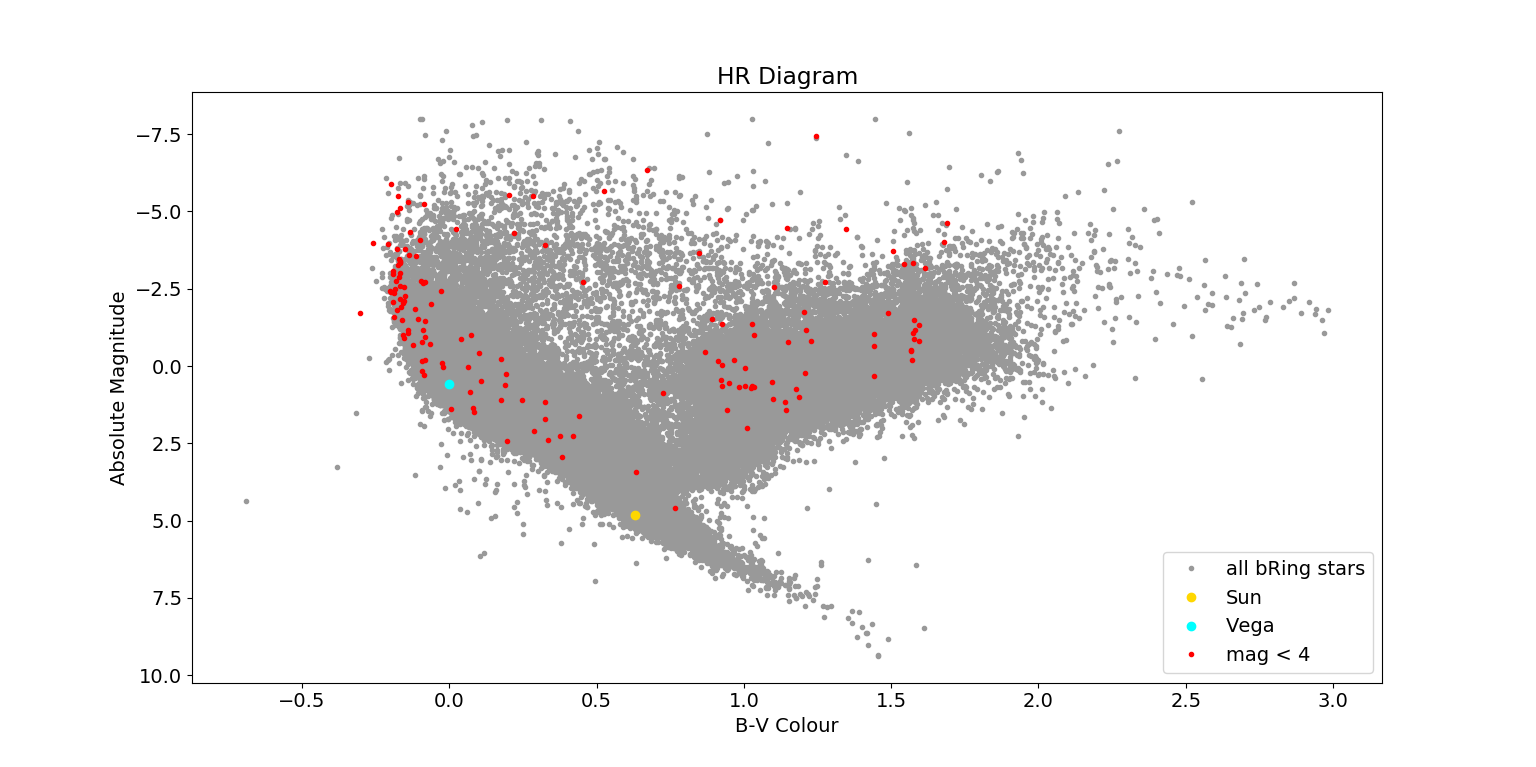
\includegraphics[width=\textwidth]{figures/HR_final.png}
    \caption{This plot presents 154 of the 157 stars for which we make light curves in red.
      %
      The grey dots represent all of the stars which are observed by bRing.
      %
      The Sun is plotted in yellow and Vega in light blue (both of which are not observed by bRing).
      %
      On the vertical axis the absolute magnitude is displayed and on the horizontal axis the B-V colour scale is shown.}
    \label{HRD}
  \end{figure}


  

  Our data set contains multiple types of variable stars, which are described in \cite{Samus_2004}.
  %
  Variable stars can be divided in two categories: intrinsic and extrinsic variables.
  %
  Intrinsic variables change in brightness because of processes inside the star, like pulsating stars and eruptive variables, for instance.
  %
  Extrinsic variability is caused by external effects, for example by eclipses or rotation of the star.

  A noticeable portion of our stars are pulsating stars.
  %
  Pulsating stars expand and shrink, most times with a certain frequency. The gravitational force and radiation pressure in the star combat each other around hydrostatic equilibrium. As the star expands, the radiation pressure weakens, causing the star to shrink. As it becomes smaller, the radiation pressure increases. This causes the star to expand once again, repeating the cycle. As it pulsates, it emits more or less light, repeatedly.
Well-known pulsating stars are Cepheids, whose period is regular and related to their luminosity. Cepheids generally pulsate radially, which means that the whole star expands and contracts evenly. Other stars may pulsate non-radially, meaning that one part of the star expands while the other part shrinks. Beta Cephei variables are main-sequence stars, while Delta Cepheids are found on the instability strip, an evolutionary stage after the main sequence.

Pulsating giant or supergiant stars that have irregular periods ranging from weeks to years are known as long period variables. These are found on the right side of the HR diagram. Long period variables with regular periods are called Mira Ceti-type variables. 

A few stars in our sample are rotating or eruptive stars. Rotating variables appear fainter or brighter when star spots come into view. These spots are cooler or warmer than the rest of the star, resulting in less or more light being emitted. Rotating stars can be main-sequence stars as well as giant stars, depending on which type of rotating star they are. Eruptive variables change in brightness irregularly due to eruptions on the surface of the star due to flares, for example. Some eruptive variables rotate as well, causing them to lose mass and appear fainter in consequence. These stars are called Gamma Cassiopeiae variables, which are all located on the main sequence in our data set. 

Our sample contains a few eclipsing binaries as well. These are systems of multiple stars, which move in front of each other from our point of view and block the light of their companion. Depending on the combination of stars, a primary eclipse as well as a secondary eclipse can be seen. As one star moves in front of the other, part of the combined emitted light is obscured. When a fainter star moves in front of the brighter star, a primary eclipse occurs. The smaller eclipse is called a secondary eclipse, which takes place when the fainter star is covered by the brighter star.\\
Binary stars can be found in a wide range of ages and sizes, but their inclination and relative size determines whether eclipses can be seen. This means that they cannot be seen at an explicit position in the HR diagram.



\section{Methods}
\label{sec:methods}
\subsection{bRing}
The bRing project is based on the MASCARA project \citep{mascara} which takes images of the sky above airmass 2. However, while MASCARA uses five CCDs (facing north, south, east, west and central) to take images of the whole visible sky in the northern hemisphere, bRing uses only two (facing east and west). The bRing telescopes are situated in Australia and South Africa, thus positioned to look at the southern hemisphere ($\delta \leq -30 \degr $). The primary goal of the two projects also differs: MASCARA was created to search for transiting exoplanets around bright stars ($4 < m_V < 8$) and bRing was constructed to monitor the Hill sphere transit of exoplanet $\beta$ Pictoris b in front of the star $\beta$ Pictoris. The transit took place from April 2017 lasting 300 days until March 2018 \citep{Wang_2016}. Because of this period bRing started collecting data on 17 January 2017 \citep{bring}. Since this day data has been collected every night.

While observing $\beta$ Pictoris, bRing observes 20000 additional bright stars, because of the wide field of view ($\approx 53\degr$ ) around the star. The bRing project also monitors the atmospheric transmission and clouds. To capture both bright and relatively fainter stars, bRing uses two exposures times: 6.38 s for relatively faint stars ($4 < m_V < 8$) and 2.54 s for the brightest stars ($m_V < 4$). This results in a total of 13500 data points per day. These data points are calibrated every night by the bRing Control Software and sent to Leiden, the Netherlands.

\begin{figure}
    \centering
    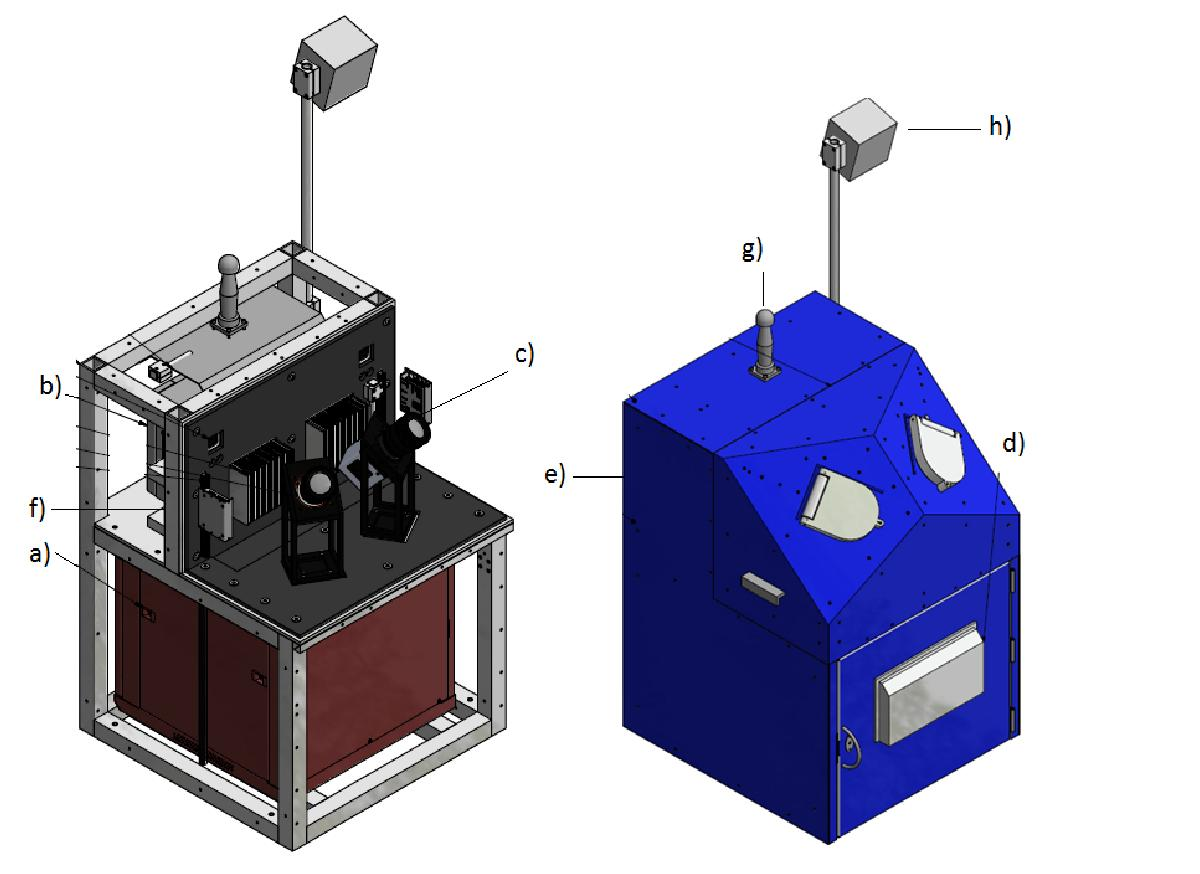
\includegraphics[width=0.65\textwidth]{figures/bRing.jpg}
    \caption{The bRing instrument. Reprinted from \cite{bring}, figure 5.}
    \label{bRing}
\end{figure}


\subsection{Data reduction}
To make long-term light curves, we started with data reduction, which we wrote using Python 2.7.
The data reduction consists of multiple steps. For each step, we used the data of one of the 4 bRing cameras at a time. The primary calibration from \cite{Talens_2018} was applied.

We used two data sets which are described as ``daily" data and ``quarterly" data. The daily data consists of all data points collected by the bRing cameras. The quarterly data bins every 50 data points, resulting in at least 50 times fewer data points compared to the daily data. We mostly used the daily data, because bright stars have very little quarterly data. Because of saturation, these stars usually do not have enough data points to be binned. 

For a star with no variability, the light curve is expected to be flat, because the amount of observed light is not expected to change. In reality, noise occurs because of outside effects such as clouds passing over the sky. This results in a distribution of data points around the mean value. To determine whether a data point should be rejected, the standard deviation was used. When removing data points based on standard deviation, we used the Astropy function \texttt{sigma\_clip}. The mean of the data set was calculated iteratively, discarding outliers each time. Based on the final calculated mean, outliers were removed from the data set. We also used this sigma-clipped-mean in further calculations when needed, instead of the mean which can be calculated before sigma-clipping.

We started the data reduction by selecting good data points from the daily and quarterly data. 
\begin{itemize}
    \item First, the long exposures were discarded. Only the short exposures were used, because the long exposures can only be used to observe stars fainter than magnitude 4. This is due to the fact that images taken with long exposure times have a higher chance of being saturated than the short exposures.
    \item Next, we used the astrometry and photometry flags of the daily data. These tell us if the measured flux is too high or too low to be realistic or if no photometry was performed due to the star being too close to the edge of the image, for example. Only the data without any bad flags was used. 
    \item We made sure that the magnitude error for the daily data is always greater than zero and finite, so no incorrect values are encountered.
    \item All data where the Sun is lower than $-18\degr$ was selected. This was added to ensure that the sky background did not get too bright. 
    \item Next, the data points where the cloud error was 3$\sigma$ above the mean cloud error were deleted. The 3$\sigma$ cutoff was estimated by eye. The cloud error tells us how the transmission changes over time; a big change might mean a cloud is in view. These outliers usually indicate that the clouds are variable at that point in time, in which case the data should not be used.
\end{itemize}
After selecting the good data points for the daily and quarterly data, the daily data was calibrated. However, we cannot use the daily data to remove, for example, the clouds, because those values are only available in the quarterly data. A piece of code written by Remko Stuik was applied to transfer the missing information from the quarterly data to the daily data. 
\begin{itemize}
    \item The 5$\sigma$ outliers based on magnitude error were discarded. A big error could mean that the measurement is wrong. 
    \item The 3$\sigma$ outliers for the mean of the clouds were also removed. This results in less background noise.
    \item The final step was to reject the 5$\sigma$ outliers for the mean of the sky background. This rejection also results in less background noise.
\end{itemize}

An example showing the different steps of the data reduction on a star has been provided below.

%teveel 'show'
\begin{figure}
    \centering
    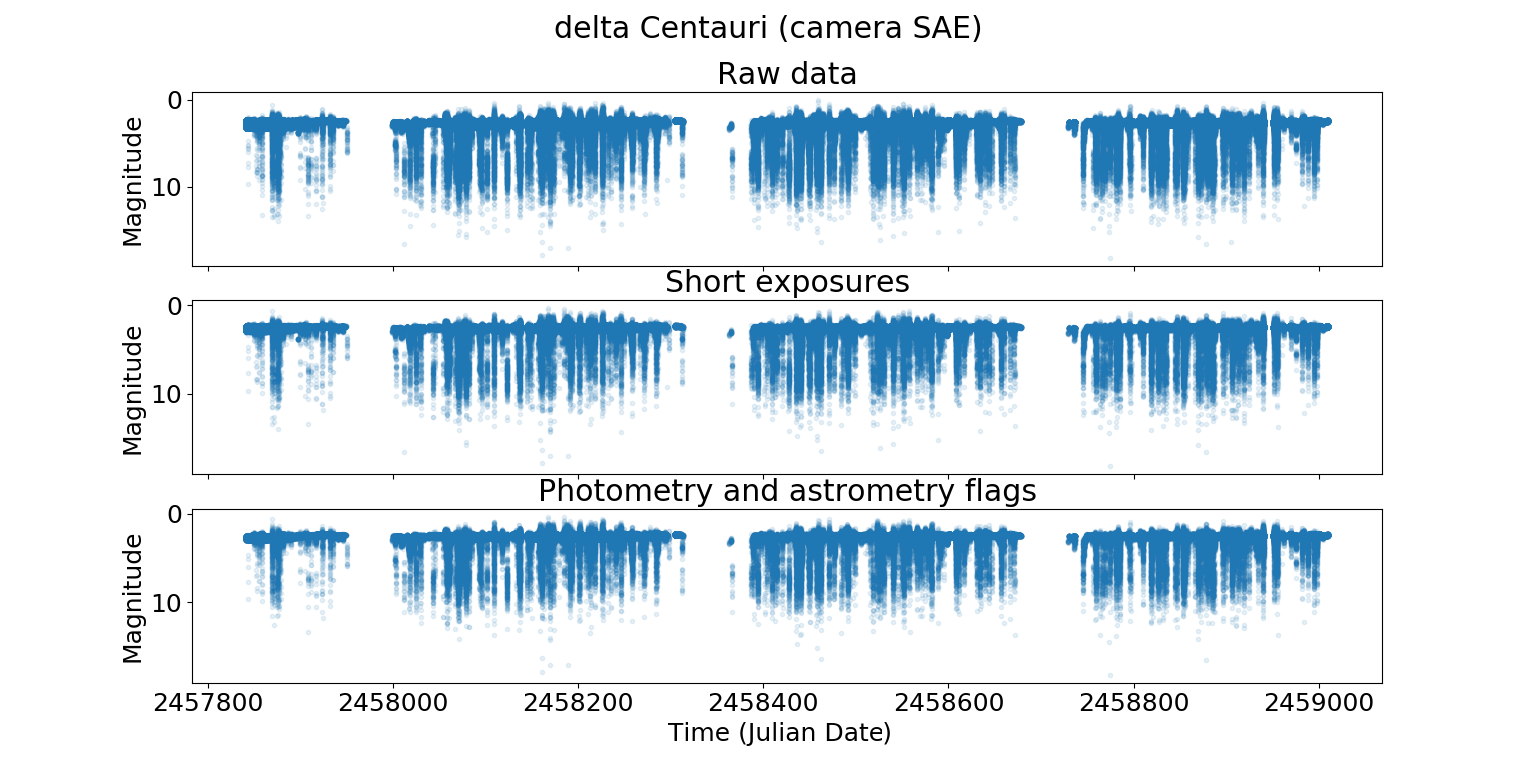
\includegraphics[width=\textwidth]{figures/delta_Cent_first3.png}
    \caption{The first three steps of the data reduction are shown here. The first plot shows the raw data that was saved by bRing. The second plot shows the data without the long exposures. Lastly, the data without the bad photometry and astrometry flags is plotted. The time is displayed on the horizontal axis in Julian Date and the apparent magnitude is displayed on the vertical axis.}
    \label{deltaCen1}
\end{figure}
\begin{figure}
    \centering
    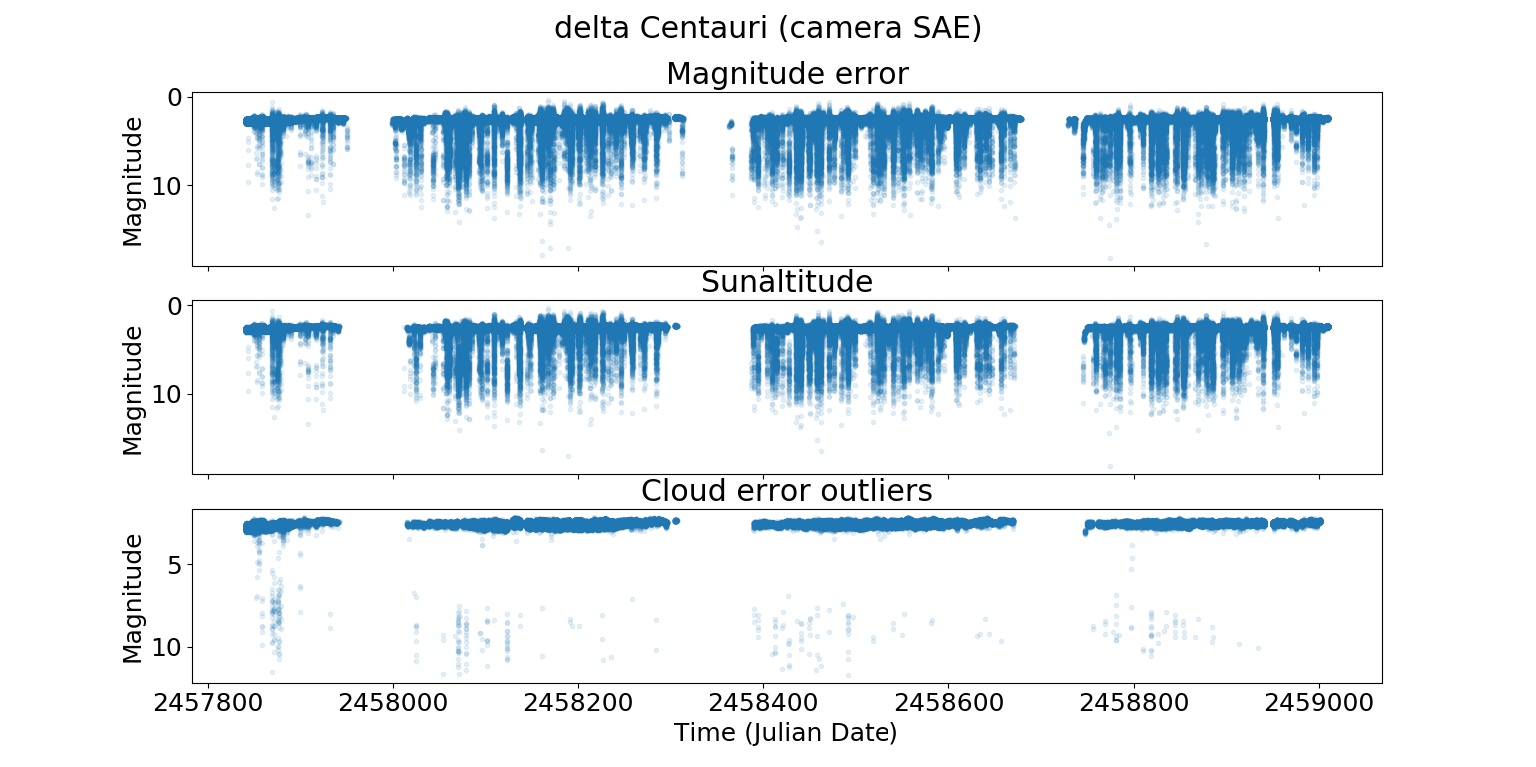
\includegraphics[width=\textwidth]{figures/delta_Cent_second3.png}
    \caption{This figure shows the next three steps of the data reduction. The first step is to make sure that the magnitude error is always finite and greater than zero. Next, the data where the altitude of the Sun is not below $-18^o$ is removed. In the last plot the 3$\sigma$ outliers on the mean of the cloud error are removed. The time is displayed on the horizontal axis in Julian Date and the apparent magnitude is displayed on the vertical axis. Note that the magnitude scale is different for the last plot.}
    \label{deltaCen2}
\end{figure}
\begin{figure}
    \centering
    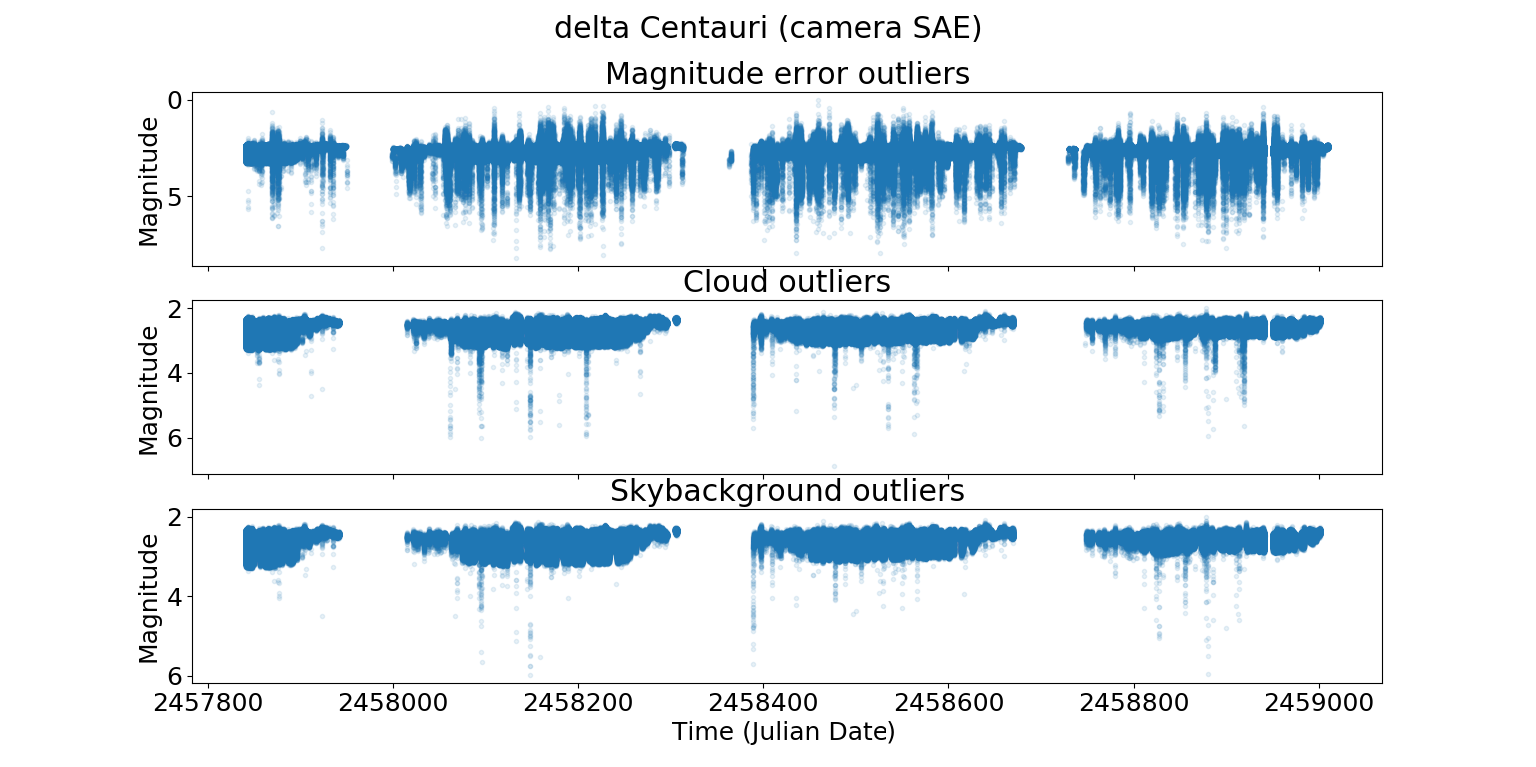
\includegraphics[width=\textwidth]{figures/delta_Cent_last3.png}
    \caption{This figure shows the last three steps of the data reduction. First, the 5$\sigma$ outliers of the mean of the magnitude error are removed. In the second plot the 3$\sigma$ outliers on the mean of the cloud are removed. Lastly, the 5$\sigma$ outliers on the sky background are removed. The time is displayed on the horizontal axis in Julian Date and the apparent magnitude is displayed on the vertical axis. Note that the magnitude scale differs for each plot.}
    \label{deltaCen3}
\end{figure}


\subsection{Detrending}
After performing data reduction, the data needed to be detrended. Detrending is the removal of trends in the data due to effects not caused by the star itself. For daily trends the effects are caused by the irregular shape of the point spread function, which changes the amount of light within the photometric aperture. For monthly trends the effects are caused by over-dimming the data points when the moon is visible.

Three trends were removed: two daily trends, and the monthly trend caused by the moon. We performed detrending similar to the secondary calibration used in \cite{Talens_2018}.

In a day, 13500 exposures can be taken in total. Every exposure at the same local sidereal time is given a number, called LSTSEQ \citep{Talens_2018}. Each night, the star should make the same path on the CCD. Detrending removes the effects caused by the same pixel receiving less or more light consistently. For every unique LSTSEQ, a sigma-clipped mean can be found. Subtracting this mean at every LSTSEQ removes this particular trend. We detrended this trend per year, because the transmission changes slightly over time.


The detrending of the second daily trend removes the effects caused by the Sun rising and setting. The sky background changes because of this. We divided a day in 500 bins, and determined the sigma-clipped mean of the data points in each bin. Each time sigma-clipping is used for detrending, the default values of 3$\sigma$, to reject data points, and 5 iterations are applied. The mean was then subtracted from all data points in one bin.

The last trend we removed is the one caused by the moon, which changes the sky background as well. The synodic period of the moon\footnote{The synodic period of the moon is 29.530588853 days.} and 25 bins per day were used to find a sigma-clipped mean per bin. This mean was subtracted from the data points in the bin. 

For each step in the detrending process, the offsets calculated in the previous step were added.

For variable stars with a known period, we detrended the data by period folding and binning, similarly to the methods described above. Period folding is the process of overlapping the data points in regular intervals. The offset gained from this step was added back in after all other detrending steps, to regain the information about a stars' period.

Examples of the detrending steps are shown in the figures below.


\begin{figure}
    \centering
    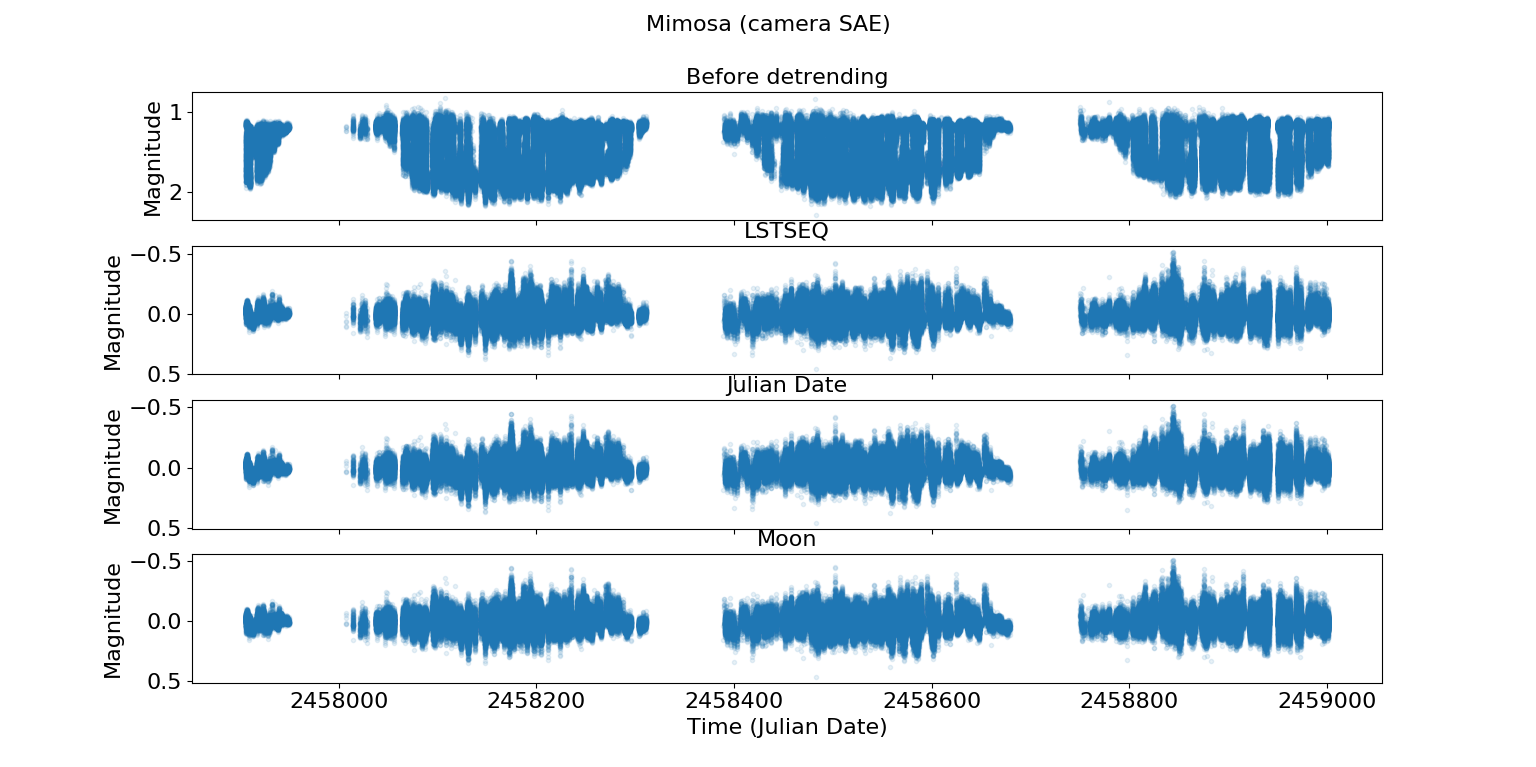
\includegraphics[width=\textwidth]{figures/Mimosa_detrend_steps.png}
    \caption{This figure shows the steps for detrending a non-variable star. The first plot shows the data before detrending.
    The second plot shows the data after detrending the LSTSEQ. The third plot shows the data after detrending per Julian Date. The final plot shows the data after detrending for the moon. The time is displayed on the horizontal axis in Julian Date and the apparent magnitude is displayed on the vertical axis.}
    \label{Mimosa_detrend_steps}
\end{figure}
%uitleg over figuren
\begin{figure}
    \centering
    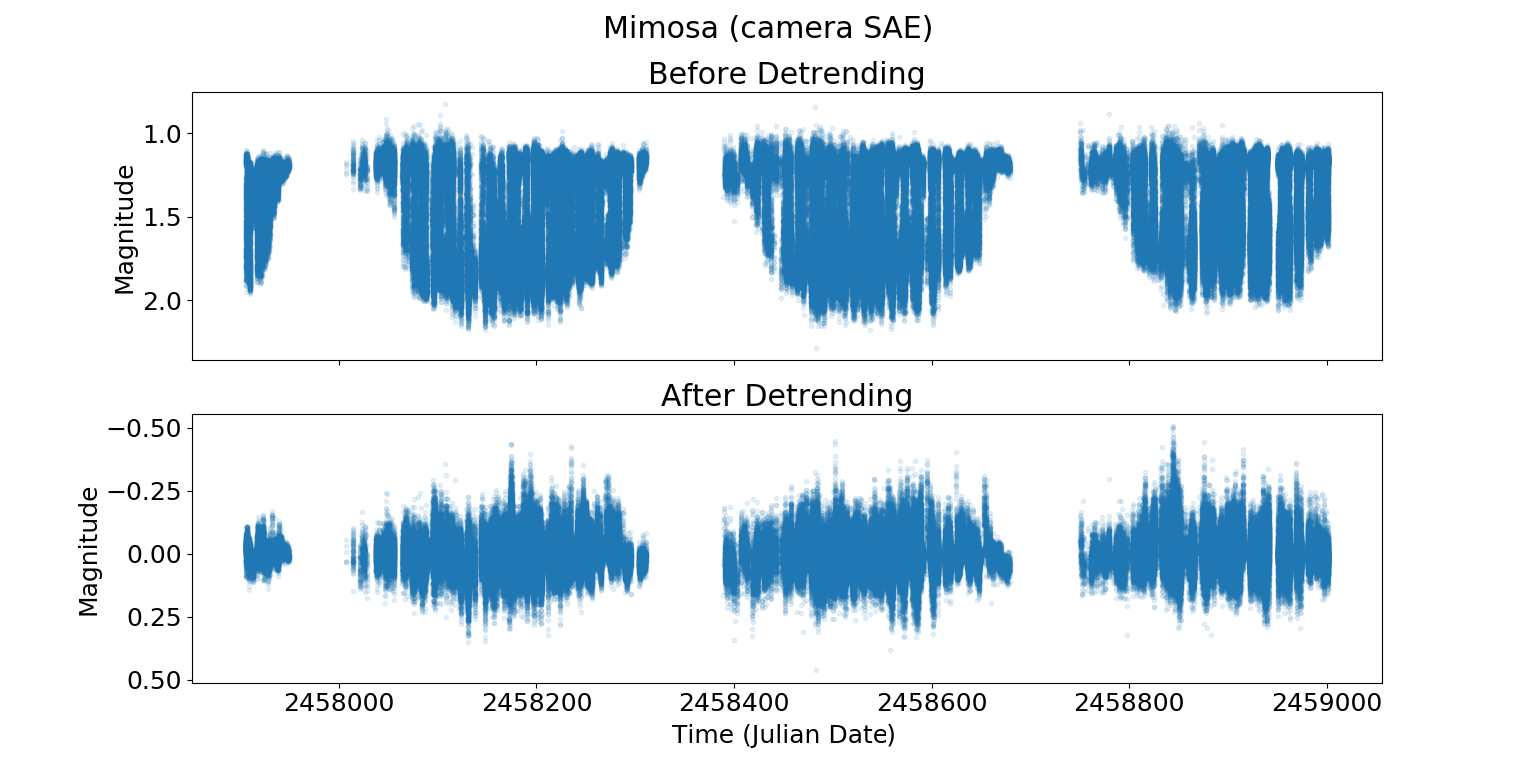
\includegraphics[width=\textwidth]{figures/Mimosa_detrending.png}
    \caption{This figure shows the difference in the light curves before and after detrending. The time is displayed on the horizontal axis in Julian Date and the apparent magnitude is displayed on the vertical axis.}
    \label{Mimosa_detrend}
\end{figure}
\begin{figure}
    \centering
    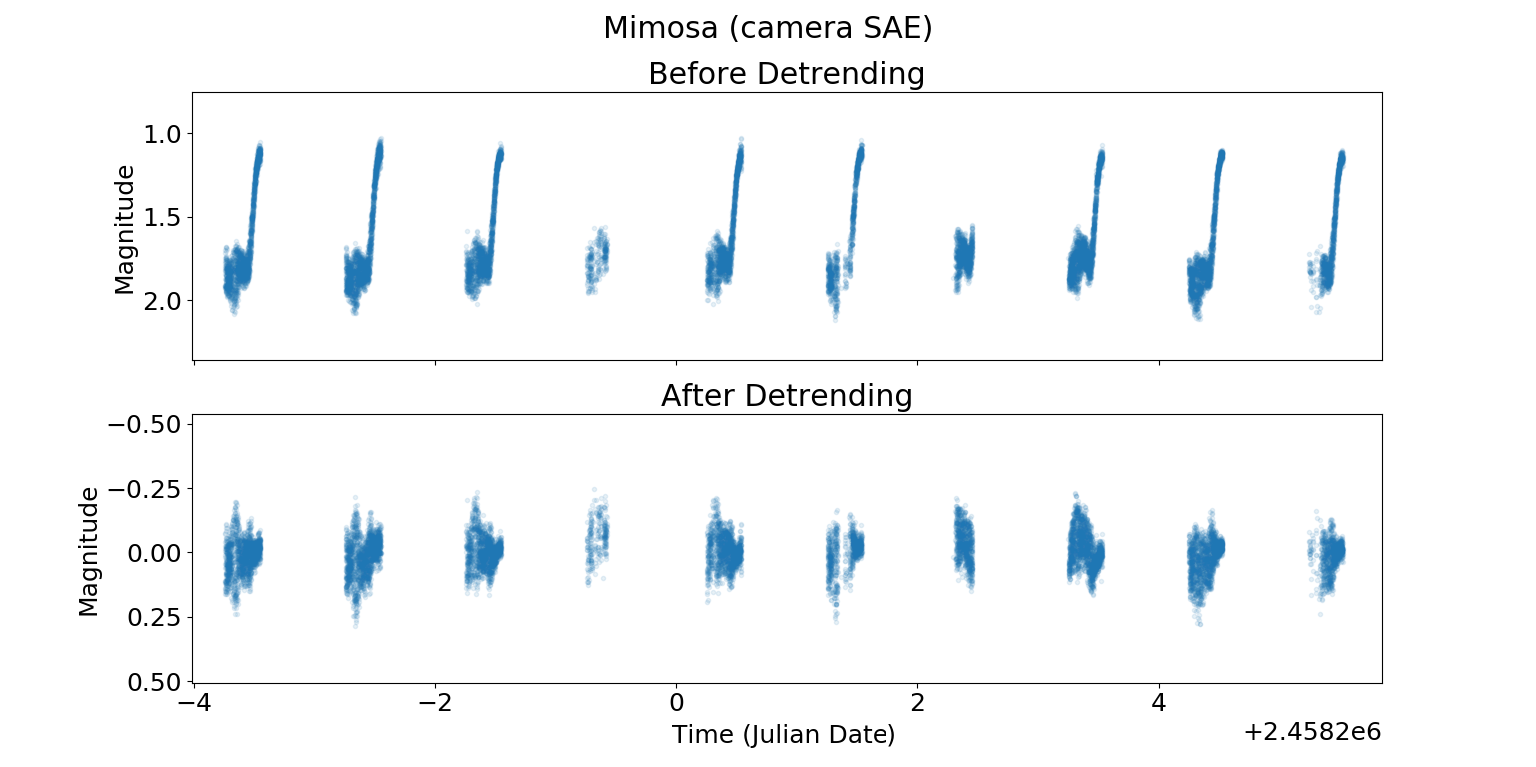
\includegraphics[width=\textwidth]{figures/Mimosa_detrending_zoom.png}
    \caption{This figure shows the difference in the light curves before and after detrending on a daily scale. The time is displayed on the horizontal axis in Julian Date and the apparent magnitude is displayed on the vertical axis. The plot is zoomed in on the horizontal axis.}
    \label{Mimosa_detrend_zoom}
\end{figure}

After detrending we bin the data to make the light curves appear more smooth. Bins of 50 data points are used, to resemble the binning of the quarterly data. Binning is conducted based on LSTSEQ, which keeps count of the possible 13500 exposures per day. This means that if two data points were taken at very different times (for example, at the end of a day and at the beginning of the next day), these points will not be put into the same bin. For every 50 points, the mean magnitude is computed. This mean magnitude is inserted at the mean time interval of the data points.


\begin{figure}
    \centering
    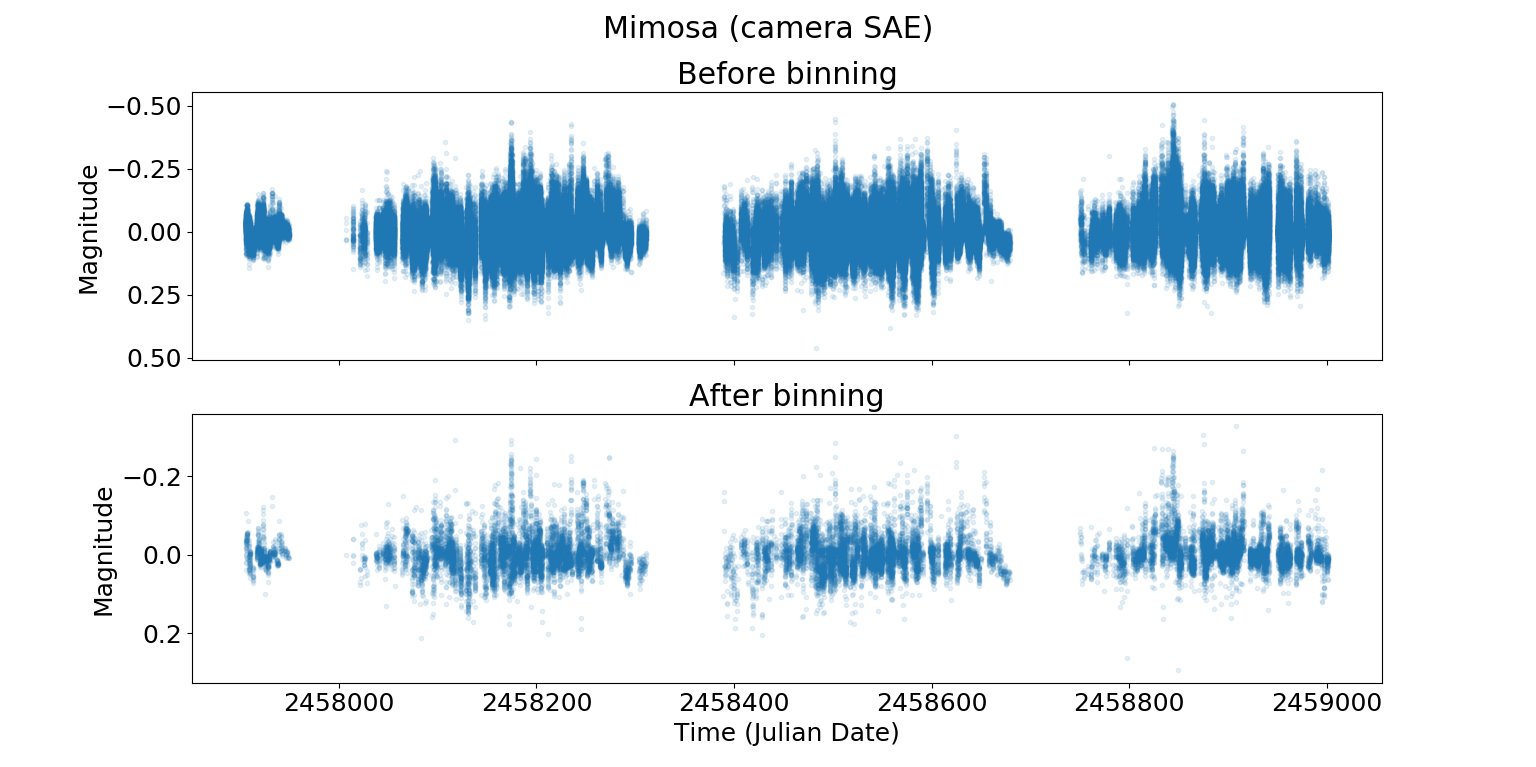
\includegraphics[width=\textwidth]{figures/Mimosa_bin.png}
    \caption{This figure shows the detrended data of a star before and after binning. The time is displayed on the horizontal axis in Julian Date and the apparent magnitude is displayed on the vertical axis.}
    \label{Mimosa_bin}
\end{figure}

\section{Searching for periodic signals}
\label{sec:tlslomb}
Using the refined light curves, periodic signals could be found. Two methods were used for this. The Transit Least Squares algorithm was used to find transits in the light curves and the Lomb-Scargle periodograms were used to find sinusoidal periodic signals in the data.

Once a signal was found, a period fold was used to determine the validity of the signal. Using a period fold, the shape of the periodic behaviour can be found.

\section{Results}
\label{sec:results}
Using the bRing cameras, the 157 brightest stars ($m_V < 4$) in the southern hemisphere were observed. After performing data reduction, the trends caused by external effects in the data were removed. This process is called detrending. We removed two daily trends and the monthly trend caused by the moon. After this, light curves of these stars were generated. Finally, periodic signals could be found using these light curves. If these signals appeared to be transits or eclipses, the Transit Least Squares algorithm \citep{Hippke_2019} was applied. For variable stars such as pulsating or rotating stars, Lomb-Scargle periodograms \citep{VanderPlas_2012} \citep{VanderPlas_2015} were used. 

\subsection{10 brightest stars}
The light curves of the ten brightest stars on the southern hemisphere are presented here, in order of decreasing brightness. 
\begin{enumerate}
\item \ref{Canopus} shows the light curve of alpha Carinae, the second brightest star in the sky and the brightest star in the southern hemisphere. It is better known as Canopus. The light curve can be seen in.
\item \ref{Rigil_Kentaurus} shows the light curve of alpha Centauri A, the third brightest stars in the sky. It is also known as Rigil Kentaurus. It is part of the alpha Centauri system, which contains Proxima Centauri, the closest star known to the Sun. 
\item \ref{Achernar} presents the light curve of alpha Eridani, also known as Achernar.
\item \ref{Hadar} shows the light curve of beta Centauri, also called Hadar. This star is a Beta Cephei.
\item \ref{Acrux} presents the light curve of alpha Crucis, a binary star system also known as Acrux.
\item \ref{Mimosa} shows the light curve of beta Crucis, also known as Mimosa.
\item \ref{Shaula} shows the light curve of lambda Scorpii, also known as Shaula. This is a binary system, with a Beta Cephei as primary star.
\item \ref{Gacrux} displays the light curve of gamma Crucis, also called Gacrux.
\item \ref{Miaplacidus} shows the ninth brightest star, beta Carinae. It is also known as Miaplacidus.
\item \ref{Alnair} shows the final brightest star. This is alpha Gruis, also known as Alnair.

\begin{figure}
    \centering
    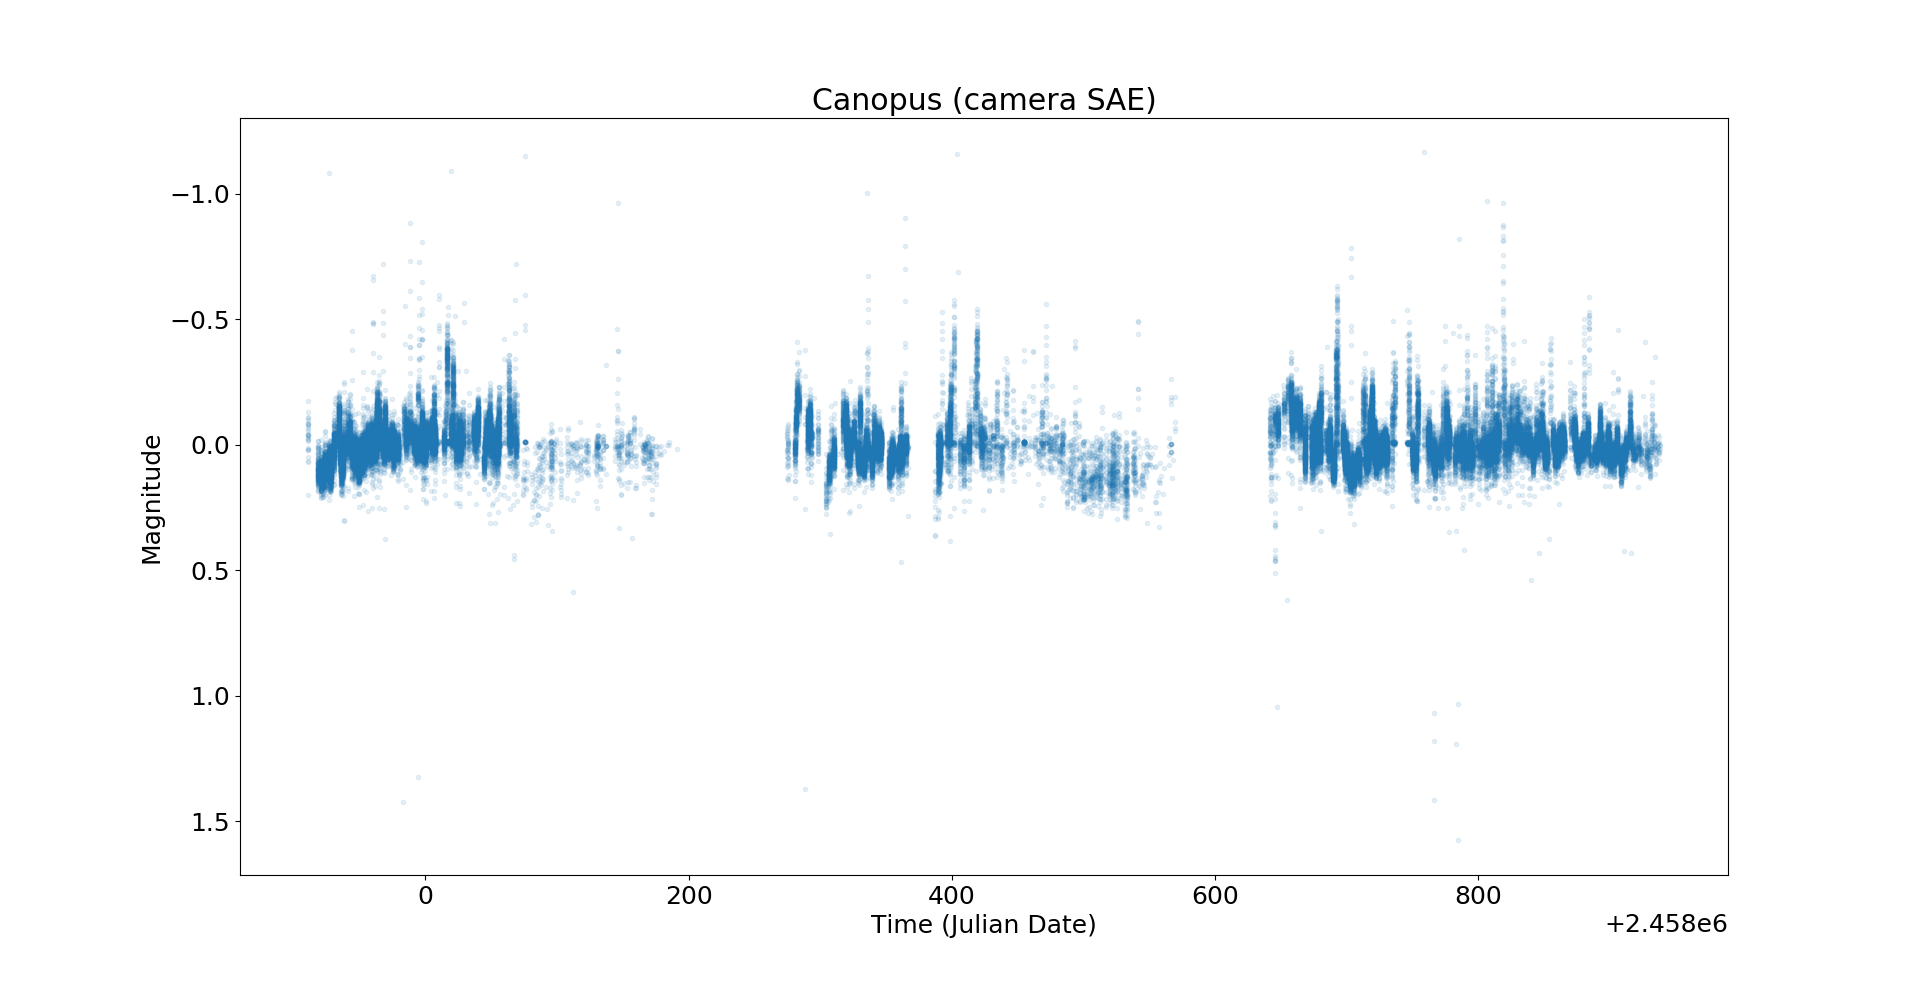
\includegraphics[width=\textwidth]{figures/Canopus_thesis.png}
    \caption{Light curve of Canopus after data reduction and detrending. The time is displayed on the horizontal axis in Julian Date and the apparent magnitude is displayed on the vertical axis. The ASCC-number of Canopus is 2111805.}
    \label{Canopus}
\end{figure}

\begin{figure}
    \centering
    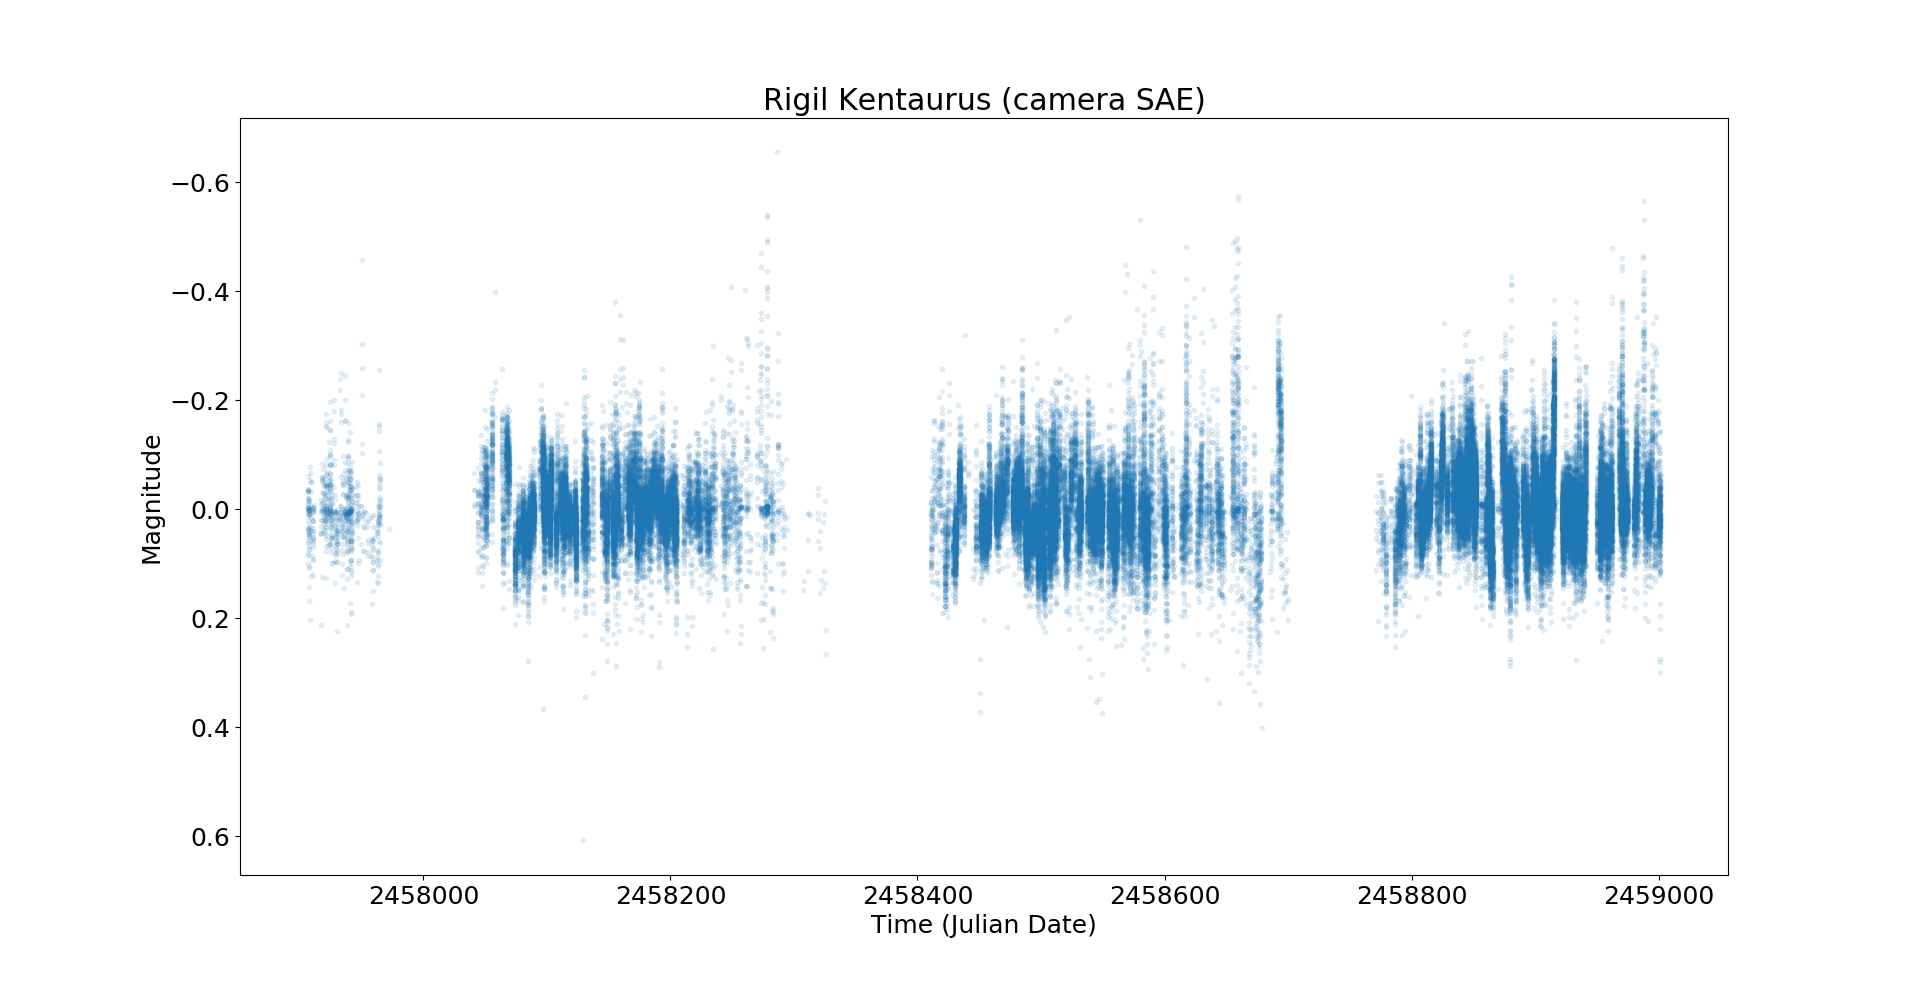
\includegraphics[width=\textwidth]{figures/Rigil_Kentaurus_thesis.png}
    \caption{Light curve of Rigil Kentaurus after data reduction and detrending. The time is displayed on the horizontal axis in Julian Date and the apparent magnitude is displayed on the vertical axis. The ASCC-number of Rigil Kentaurus is 2348878.}
    \label{Rigil_Kentaurus}
\end{figure}

\begin{figure}
    \centering
    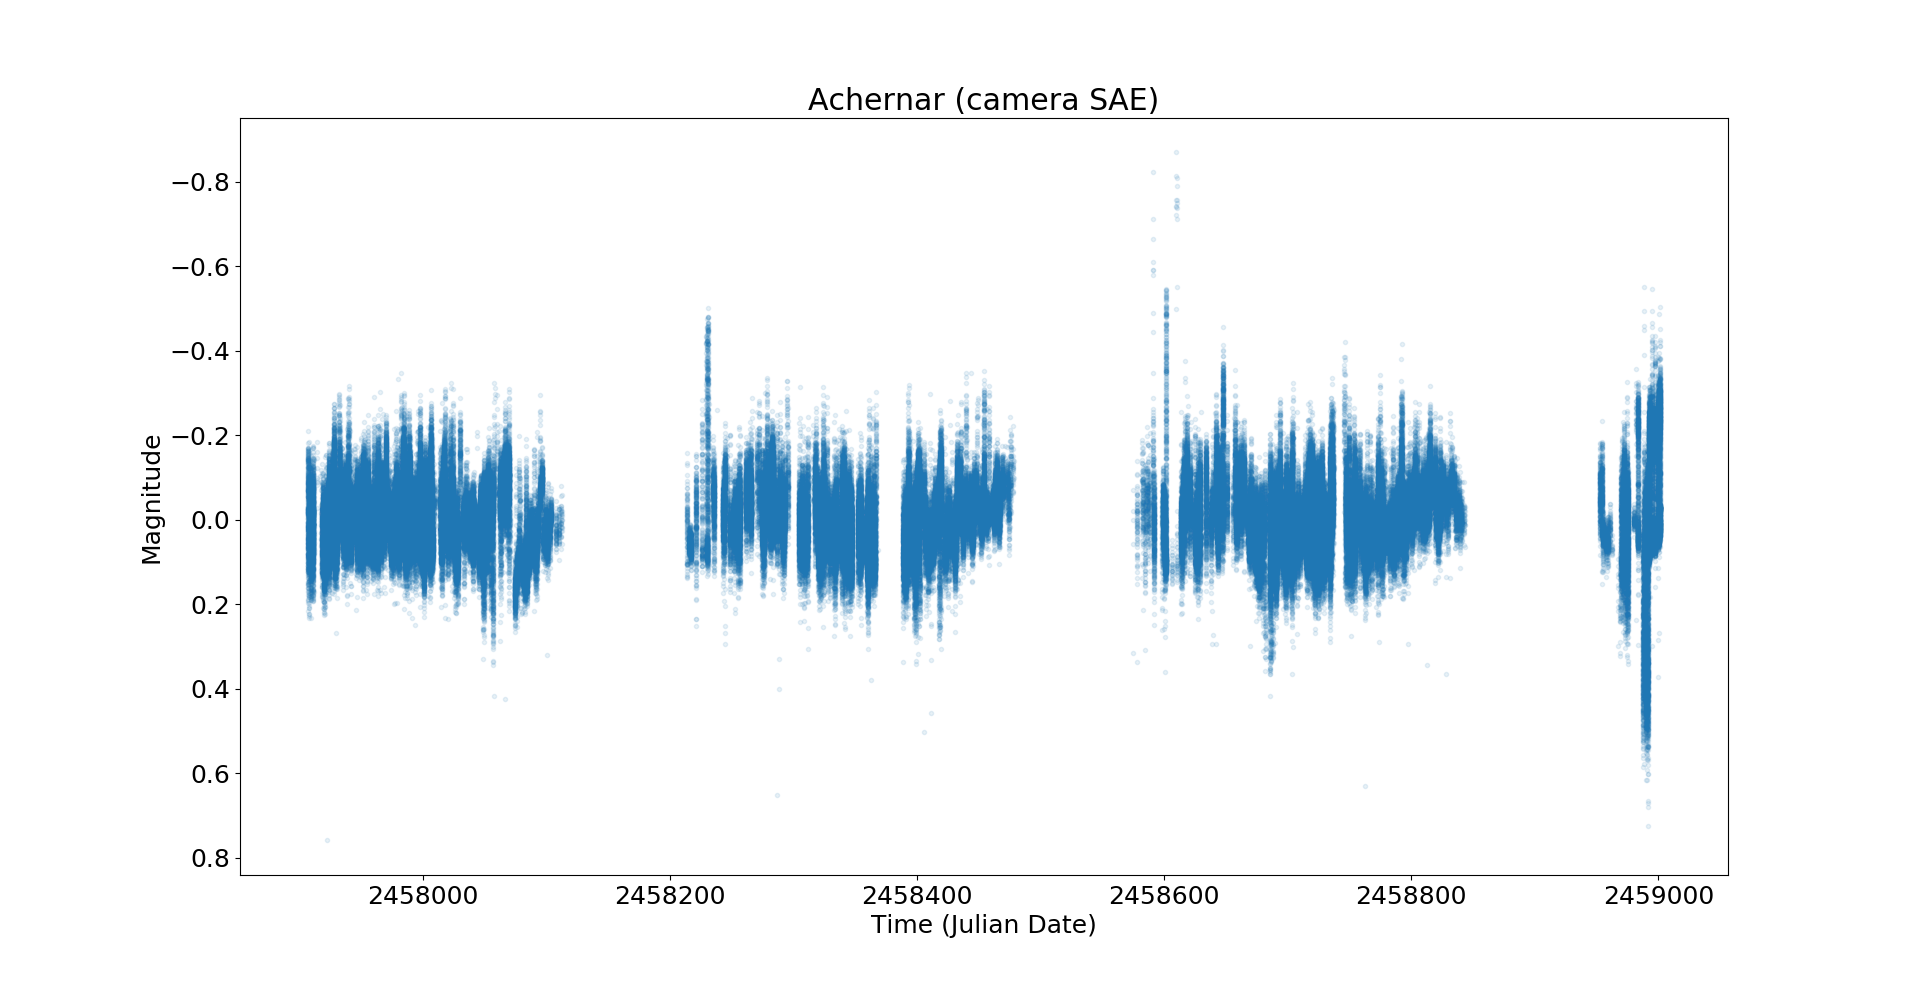
\includegraphics[width=\textwidth]{figures/Achernar_thesis.png}
    \caption{Light curve of Achernar after data reduction and detrending. The time is displayed on the horizontal axis in Julian Date and the apparent magnitude is displayed on the vertical axis. The ASCC-number of Achernar is 2199019.}
    \label{Achernar}
\end{figure}

\begin{figure}
    \centering
    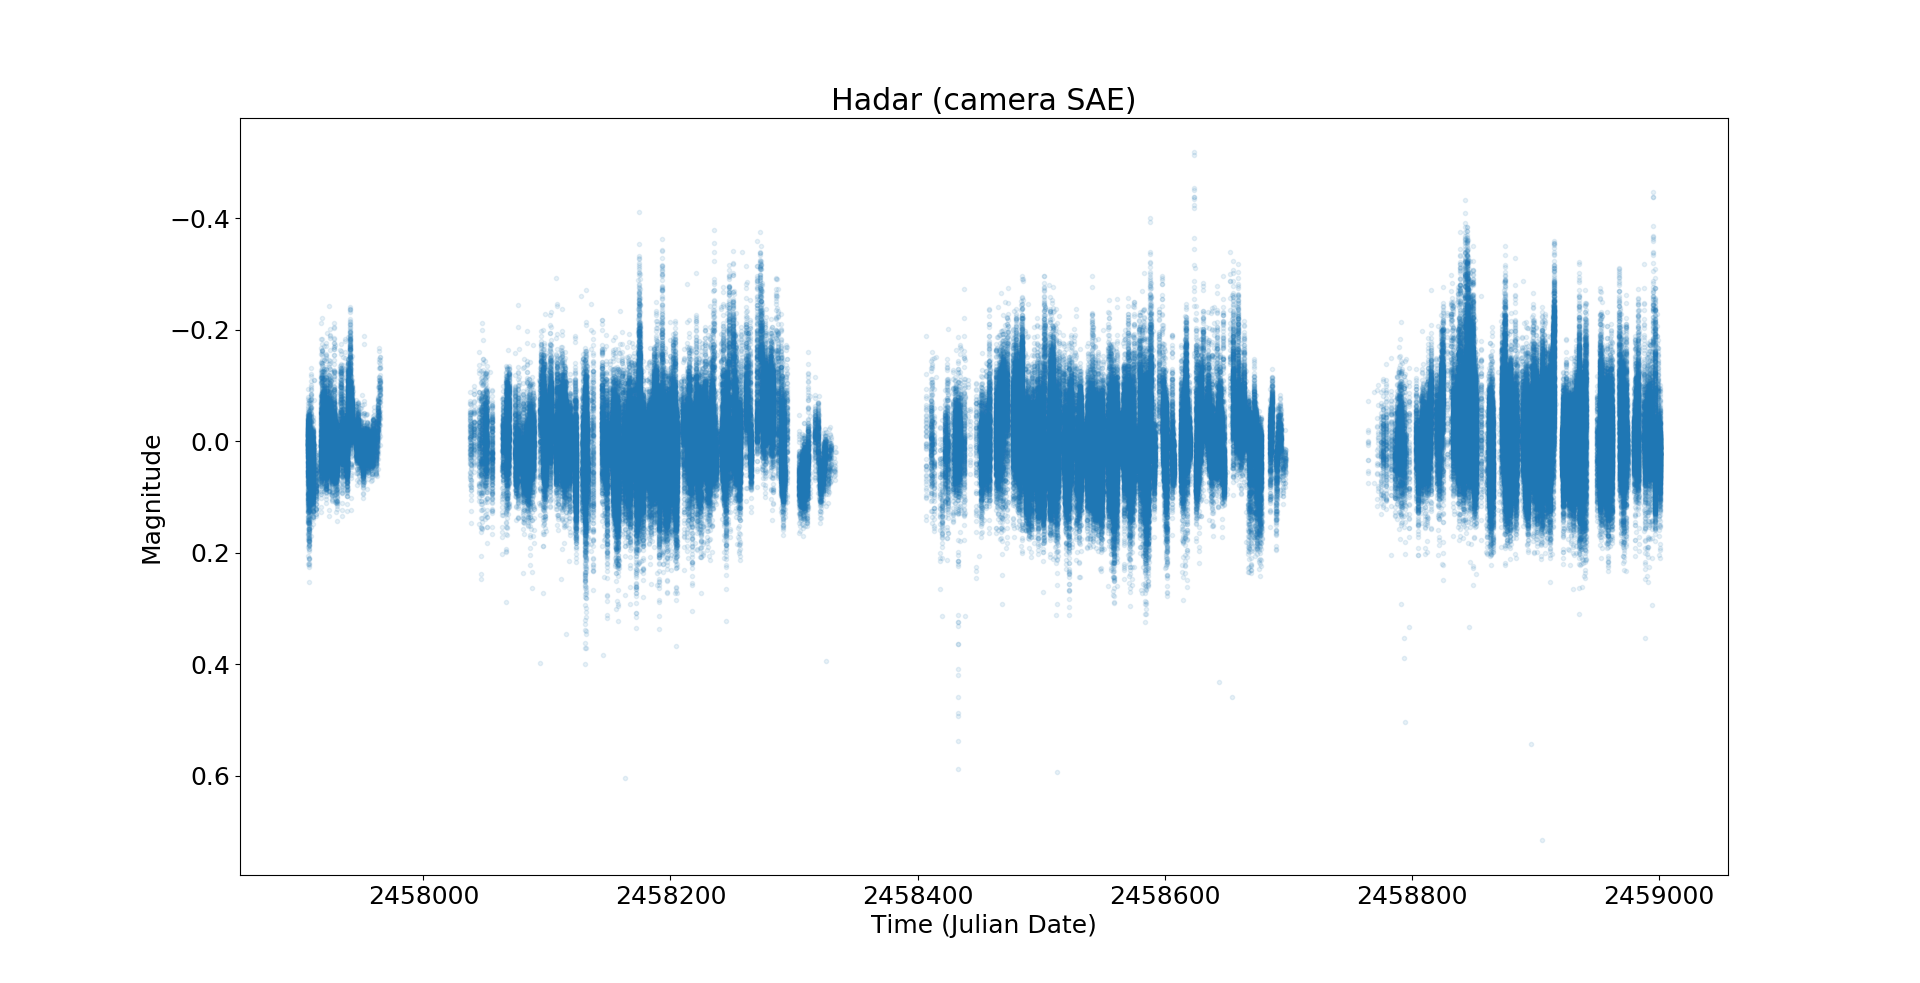
\includegraphics[width=\textwidth]{figures/Hadar_thesis.png}
    \caption{Light curve of Hadar after data reduction and detrending. The time is displayed on the horizontal axis in Julian Date and the apparent magnitude is displayed on the vertical axis. The ASCC-number of Hadar is 2345078.}
    \label{Hadar}
\end{figure}

\begin{figure}
    \centering
    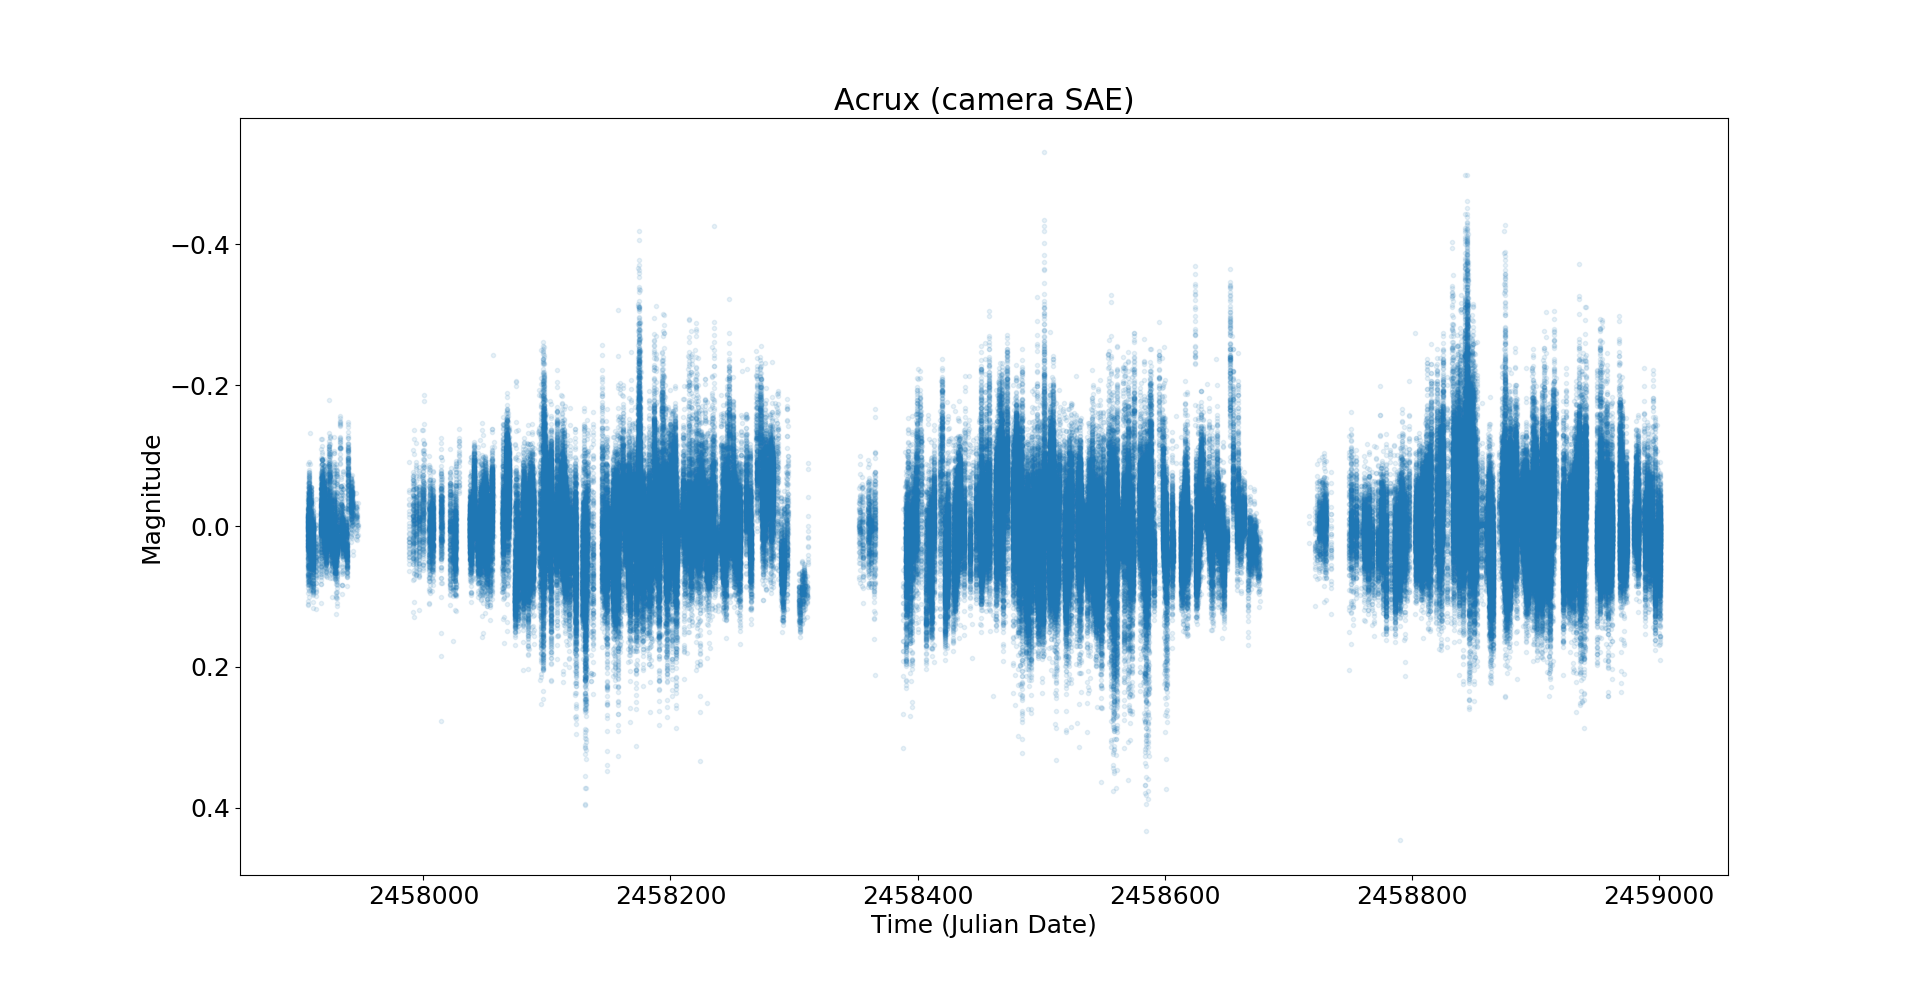
\includegraphics[width=\textwidth]{figures/Acrux_thesis.png}
    \caption{Light curve of Acrux after data reduction and detrending. The time is displayed on the horizontal axis in Julian Date and the apparent magnitude is displayed on the vertical axis. The ASCC-number of Acrux is 2333718.}
    \label{Acrux}
\end{figure}

\begin{figure}
    \centering
    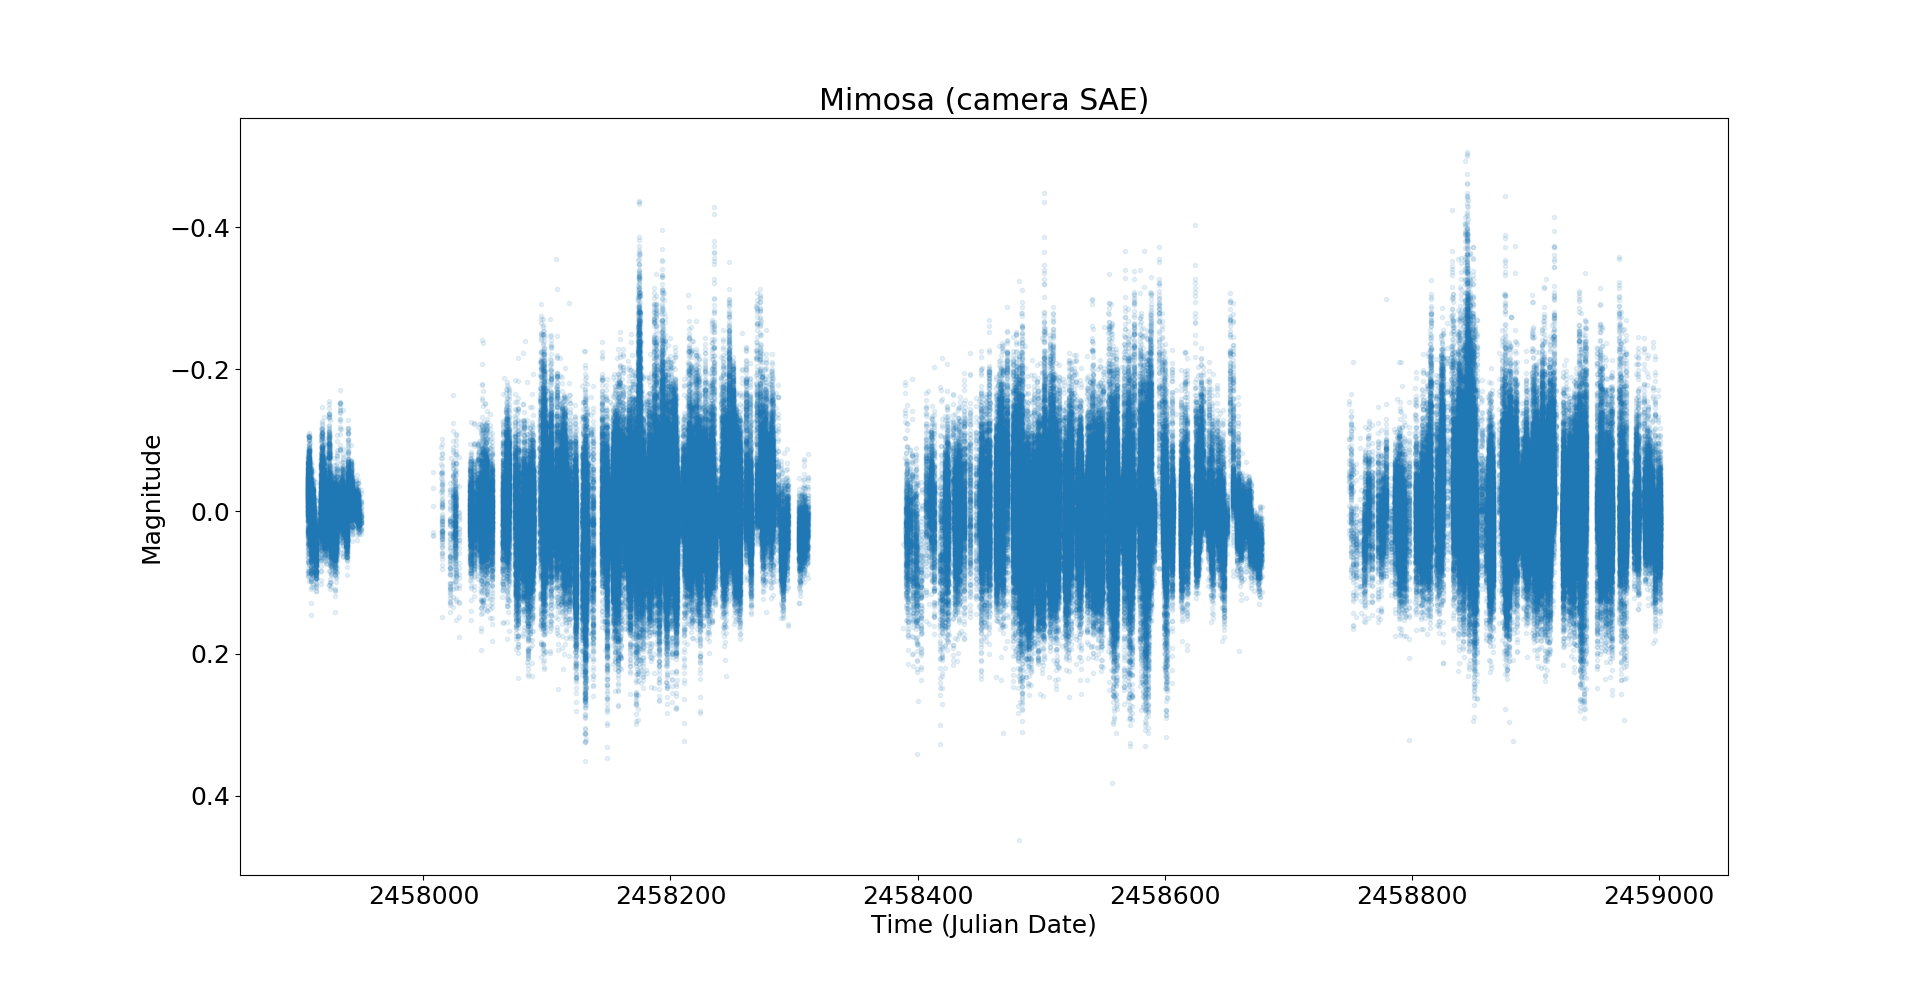
\includegraphics[width=\textwidth]{figures/Mimosa_thesis.png}
    \caption{Light curve of Mimosa after data reduction and detrending. The time is displayed on the horizontal axis in Julian Date and the apparent magnitude is displayed on the vertical axis. The ASCC-number of Mimosa is 2250231.}
    \label{Mimosa}
\end{figure}

\begin{figure}
    \centering
    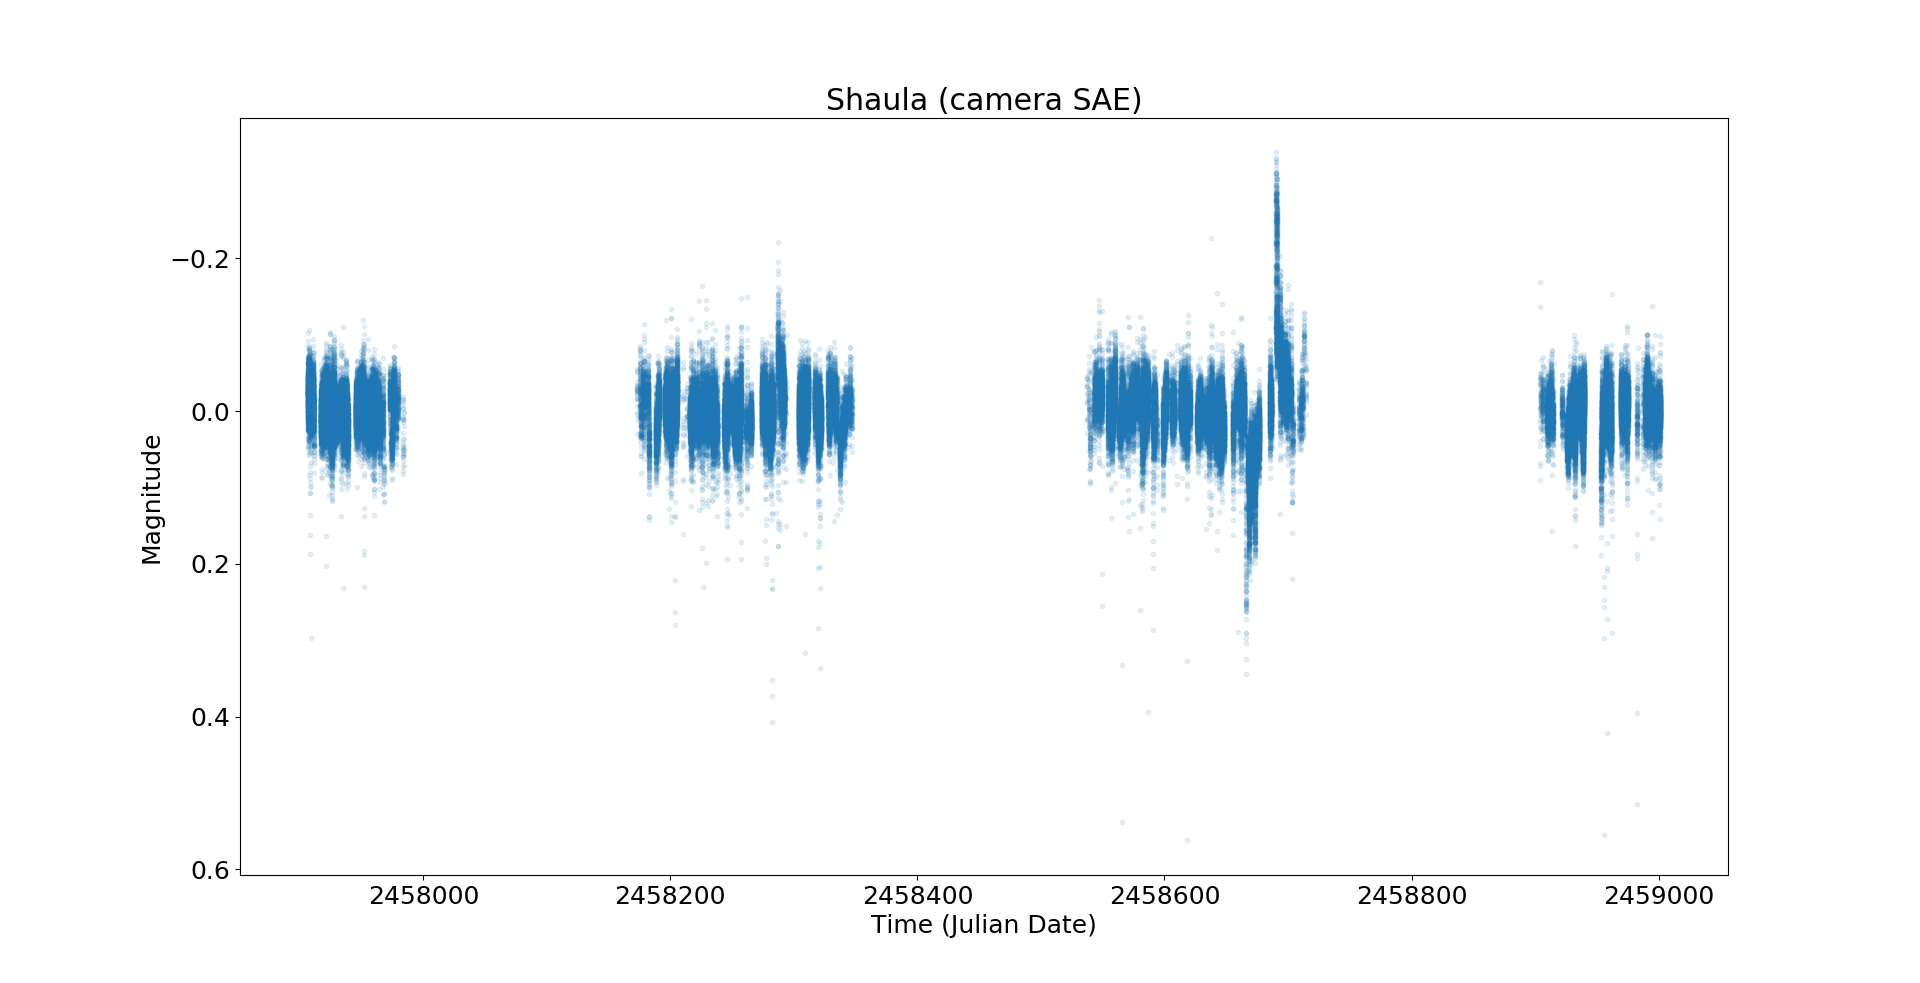
\includegraphics[width=\textwidth]{figures/Shaula_thesis.png}
    \caption{Light curve of Shaula after data reduction and detrending. The time is displayed on the horizontal axis in Julian Date and the apparent magnitude is displayed on the vertical axis. The ASCC-number of Shaula is 1880898.}
    \label{Shaula}
\end{figure}

\begin{figure}
    \centering
    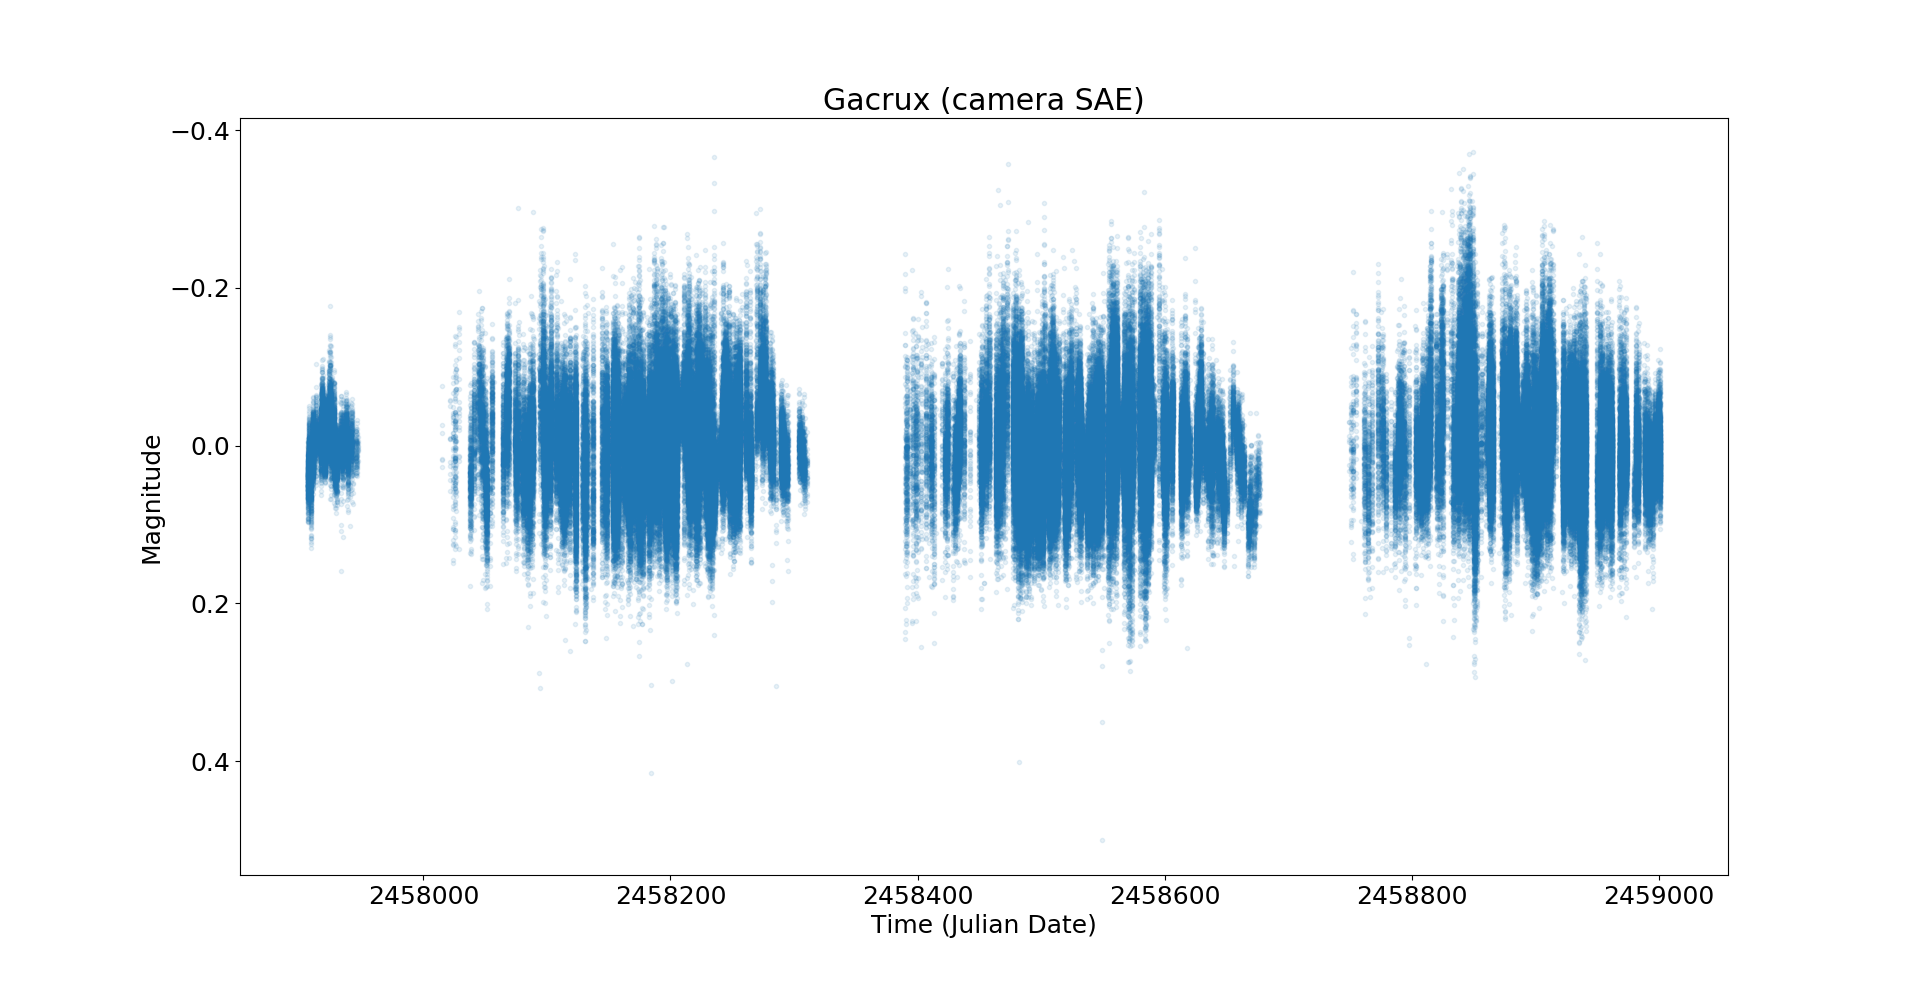
\includegraphics[width=\textwidth]{figures/Gacrux_thesis.png}
    \caption{Light curve of Gacrux after data reduction and detrending. The time is displayed on the horizontal axis in Julian Date and the apparent magnitude is displayed on the vertical axis. The ASCC-number of Gacrux is 2248482.}
    \label{Gacrux}
\end{figure}

\begin{figure}
    \centering
    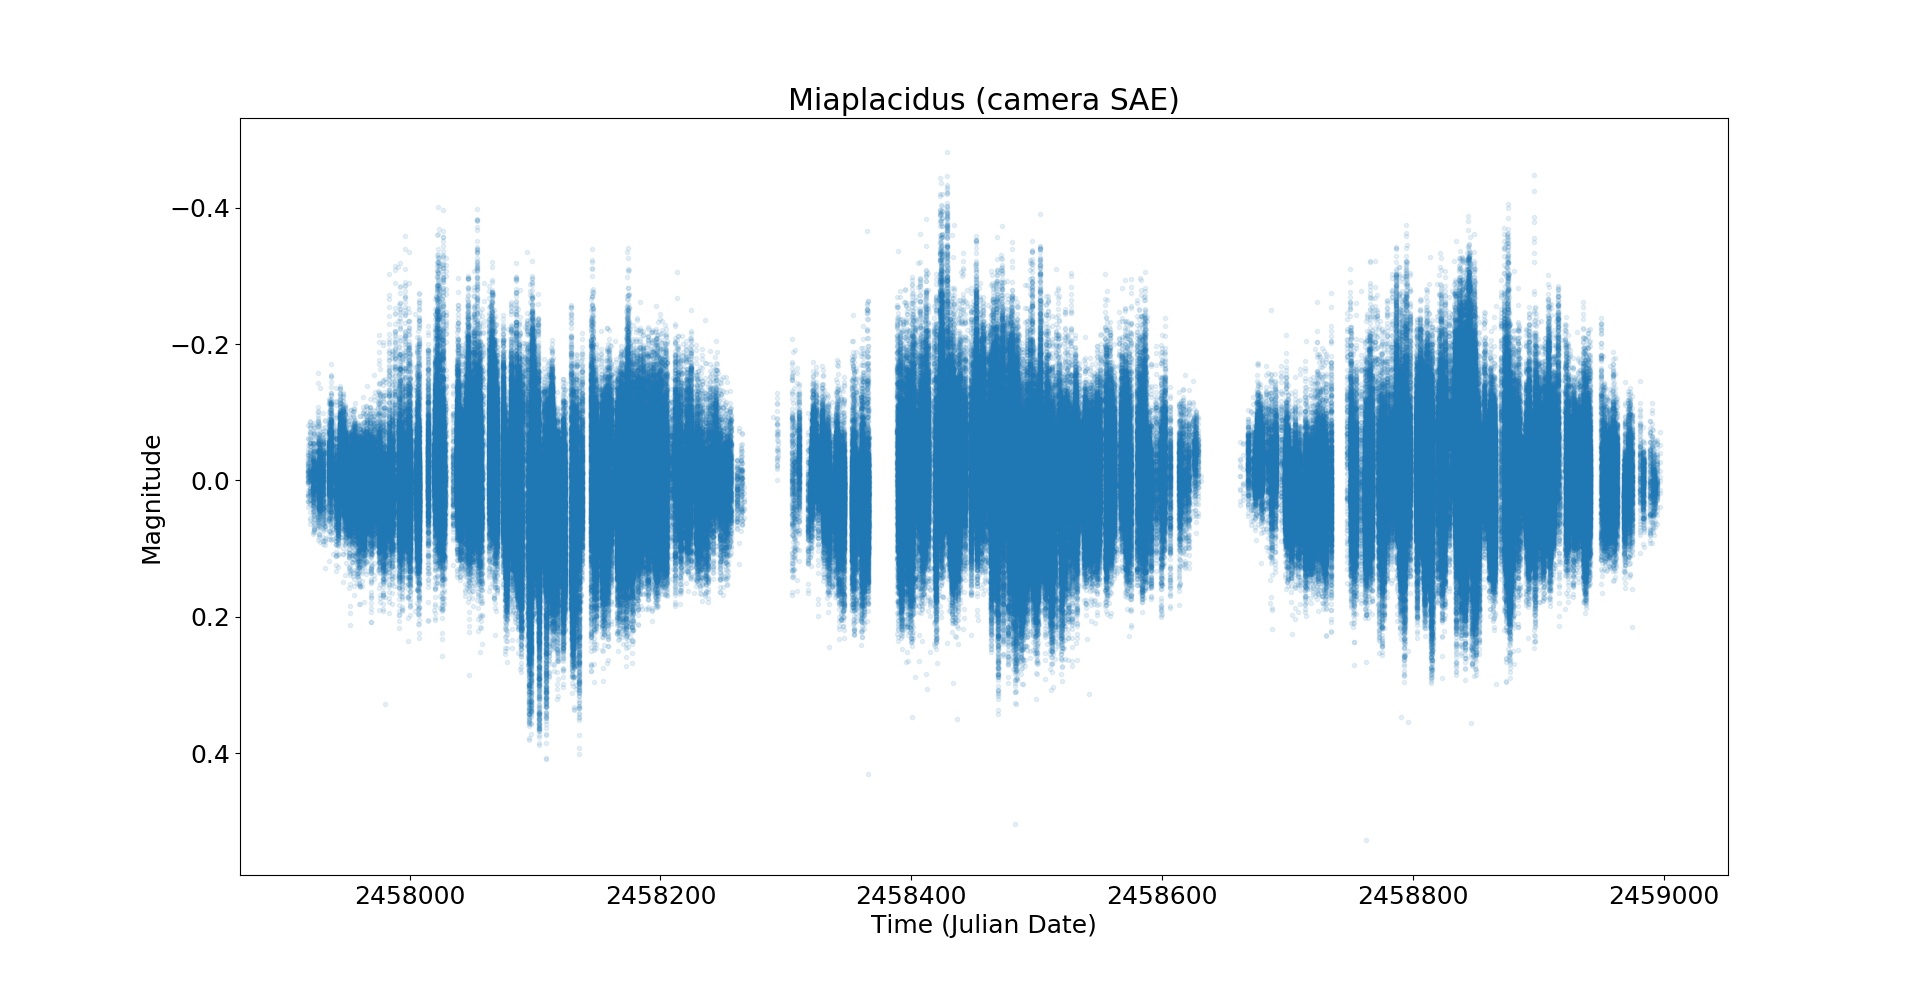
\includegraphics[width=\textwidth]{figures/Miaplacidus_thesis.png}
    \caption{Light curve of Miaplacidus after data reduction and detrending. The time is displayed on the horizontal axis in Julian Date and the apparent magnitude is displayed on the vertical axis. The ASCC-number of Miaplacidus is 2386073.}
    \label{Miaplacidus}
\end{figure}

\begin{figure}
    \centering
    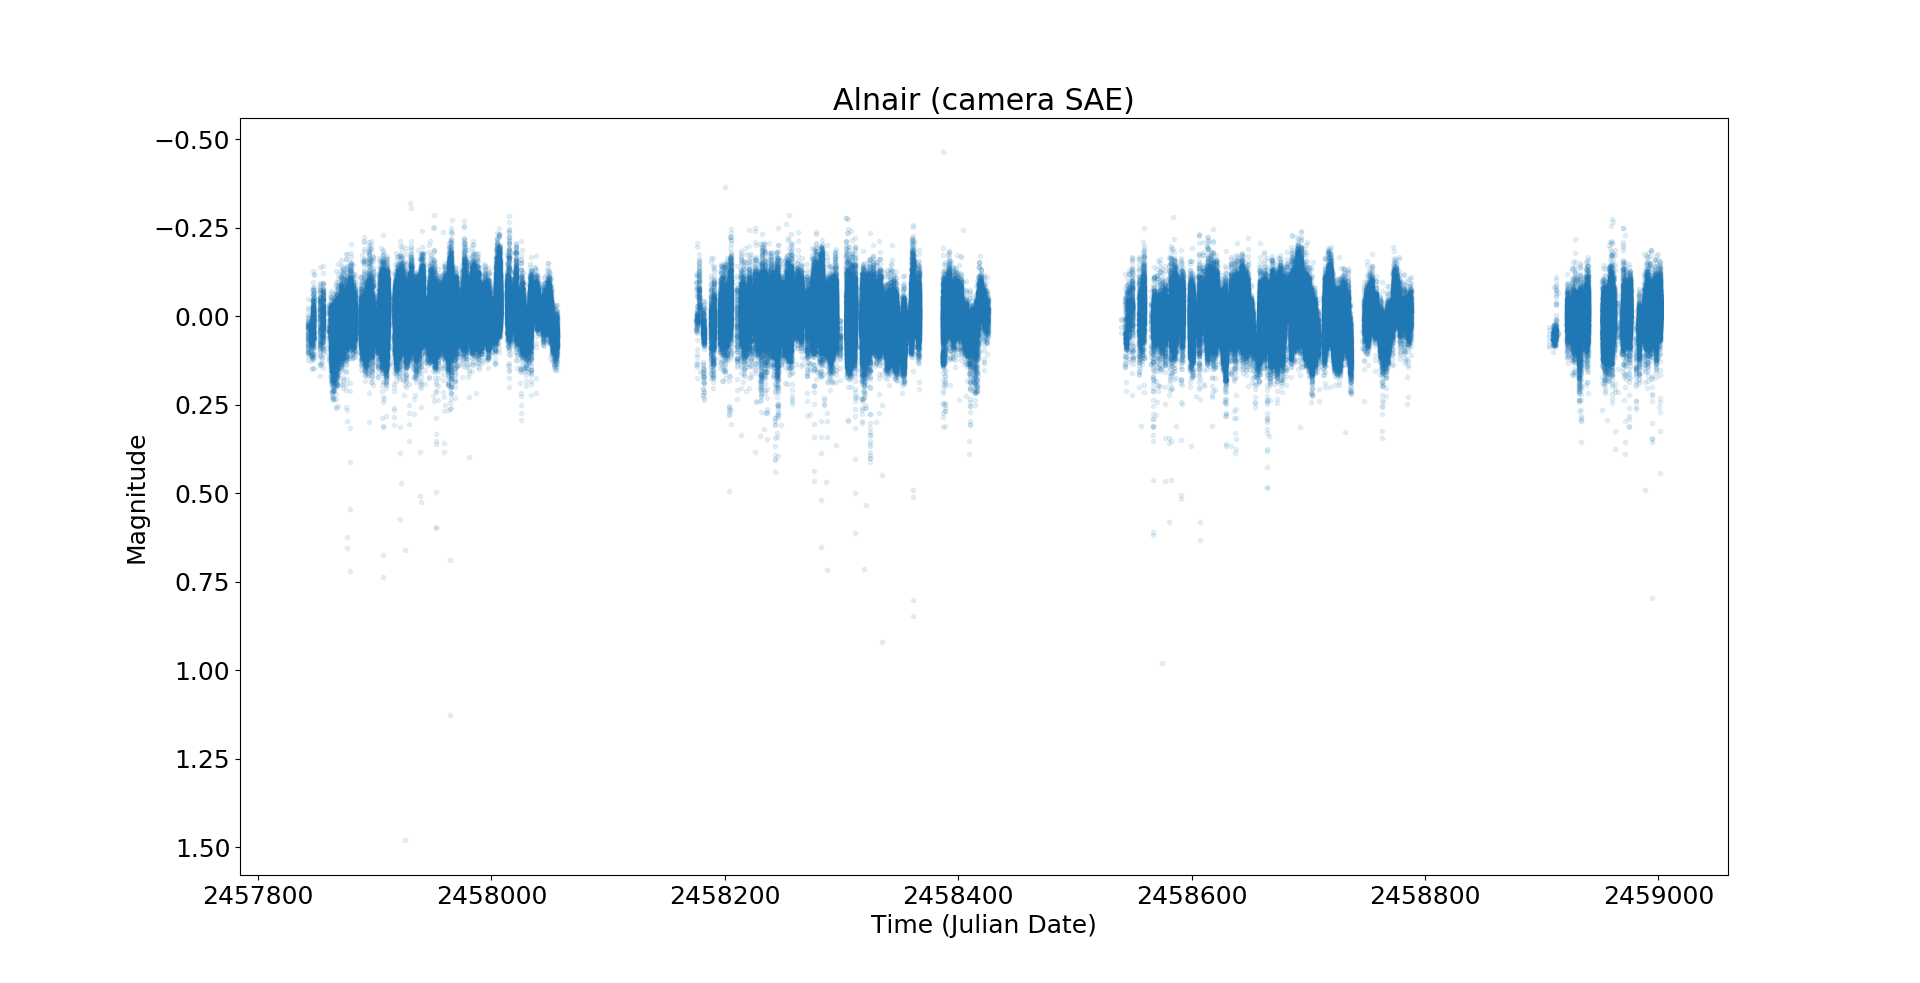
\includegraphics[width=\textwidth]{figures/Alnair_thesis.png}
    \caption{Light curve of Alnair after data reduction and detrending. The time is displayed on the horizontal axis in Julian Date and the apparent magnitude is displayed on the vertical axis. The ASCC-number of Alnair is 2098110.}
    \label{Alnair}
\end{figure}
\end{enumerate}

\subsection{Stars similar to the Sun} 
Two stars are very close to the Sun in the HR diagram in \ref{HRD}. These stars are delta Pavonis and beta Hydri. Delta Pavonis has a luminosity of 1.22 L$_\odot$ \citep{Bruntt_2010}, a mass of 0.991 M$_\odot$ and a radius of 1.22 R$_\odot$ \citep{2008yCat..21680297T}. It is a subgiant star which will relatively soon start to become a red giant. Beta Hydri has a luminosity of 3.49 L$_\odot$, a mass of 1.08 M$_\odot$ and a of radius 1.81 R$_\odot$ \citep{Brand_o_2011}. Beta Hydri is also a subgiant star. 

\begin{figure}
    \centering
    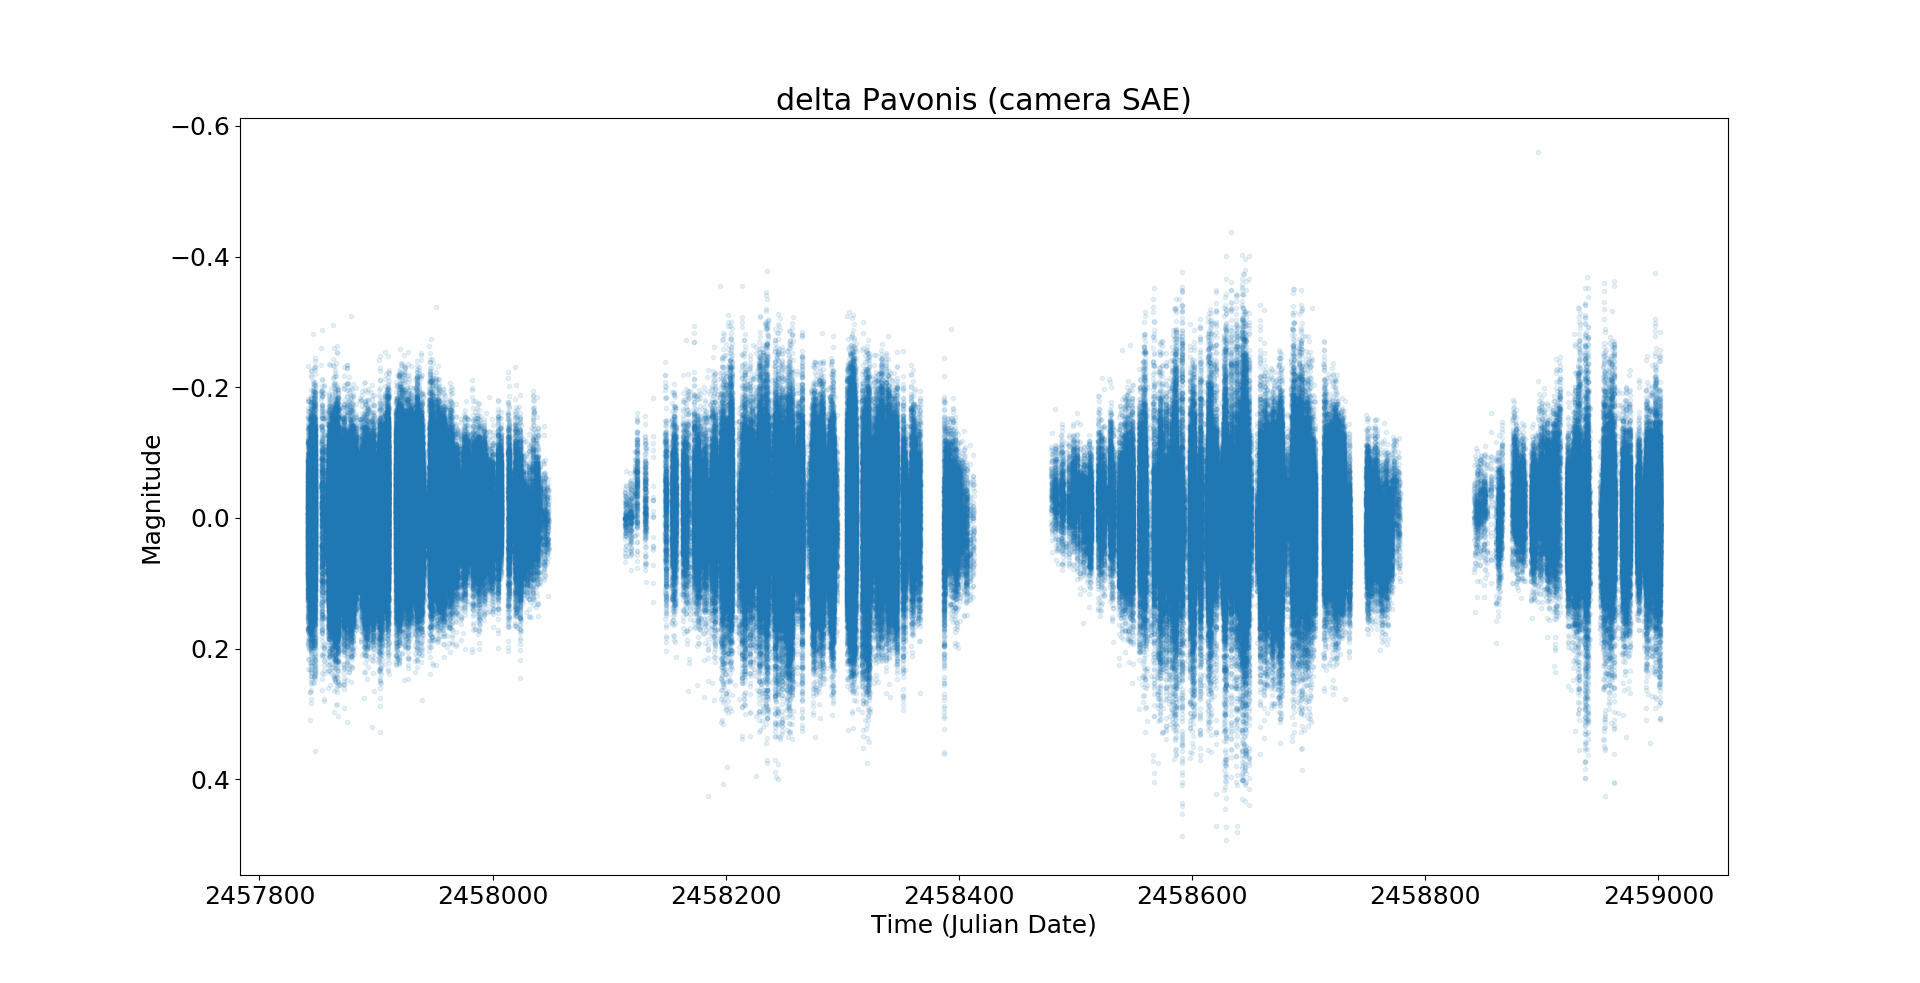
\includegraphics[width=\textwidth]{figures/del_Pav_thesis.png}
    \caption{Light curve of delta Pavonis after data reduction and detrending. The time is displayed on the horizontal axis in Julian Date and the apparent magnitude is displayed on the vertical axis. The ASCC-number of delta Pavonis is 2424942.}
    \label{del_Pav}
\end{figure}

\begin{figure}
    \centering
    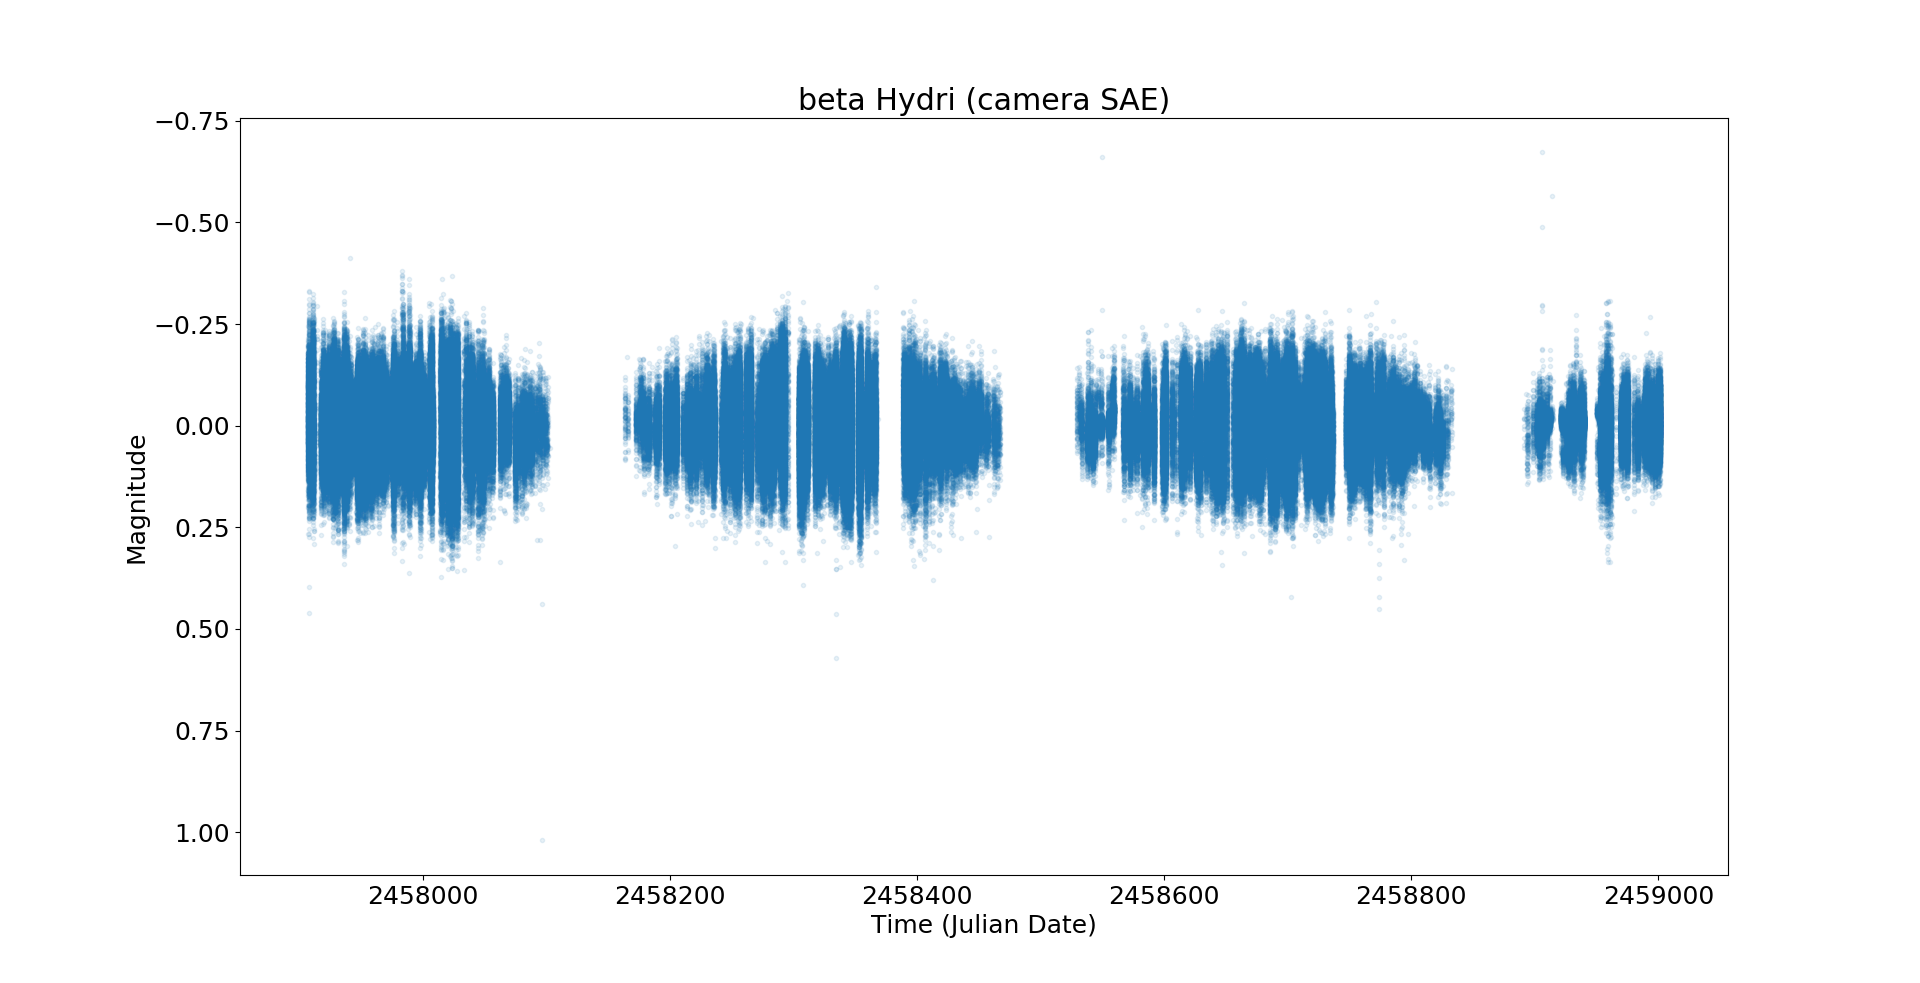
\includegraphics[width=\textwidth]{figures/bet_Hyi_thesis.png}
    \caption{Light curve of beta Hydri after data reduction and detrending. The time is displayed on the horizontal axis in Julian Date and the apparent magnitude is displayed on the vertical axis. The ASCC-number of beta Hydri is 2430714.}
    \label{bet_Hyi}
  \end{figure}


  
\section{Discussion}
\label{sec:discussion}

157 light curves of the brightest stars ($m_V < 4$) in the southern hemisphere ($\delta \leq -30^o$) were created. This is the first time light curves have been produced for such bright stars. We discuss our results in the subsections below. Limitations and strengths of the methods used are given as well.

\subsection{Data reduction}
\label{sec:discdatared}
The data reduction still has a few shortcomings.

Normally, the last step of the data reduction would be to remove the $5 \sigma$ magnitude outliers. To remove these outliers, the mean of the magnitude should be calculated as accurately as possible. To determine this mean, the best calibrated day in the data for that star should be used. The data points for this day should lie on a horizontal line, without any clear outliers. We defined this day to have a cloud error within 0.5$\sigma$ of the mean cloud error. This constraint was chosen by eye. The day which had the most data points within the limitation should be selected.

However, a lot of data points seem to be concentrated around a magnitude value which is used to fix the mean magnitude. This value originates from the bRing catalogue \citep{Talens_2018}. The concentration of data points might be caused by a lack of data points, meaning too many will be fixed around this value. In the light curves, this can be seen as a stripe or blob of data points concentrated around a fixed value. This results in an unusually small standard deviation, making good data points seem outliers when rejecting $5\sigma$ outliers.

For some stars, removing the $5 \sigma$ outliers results in a cleaner light curve. However, for most stars, too many accurate data points are removed in this process, which can be seen in the histogram in \ref{hist}. A sharp cutoff is visible at the higher magnitudes. A peak can be seen at the magnitude value originating from the bRing database as well ($m_V = 3.848$).

If a solution to this problem is discovered in the future, it should be possible to adapt the reduced data by adding in another data reduction step. The data reduction steps taken in this research could still be used in this case, and do not have to be repeated.
\begin{figure}
    \centering
    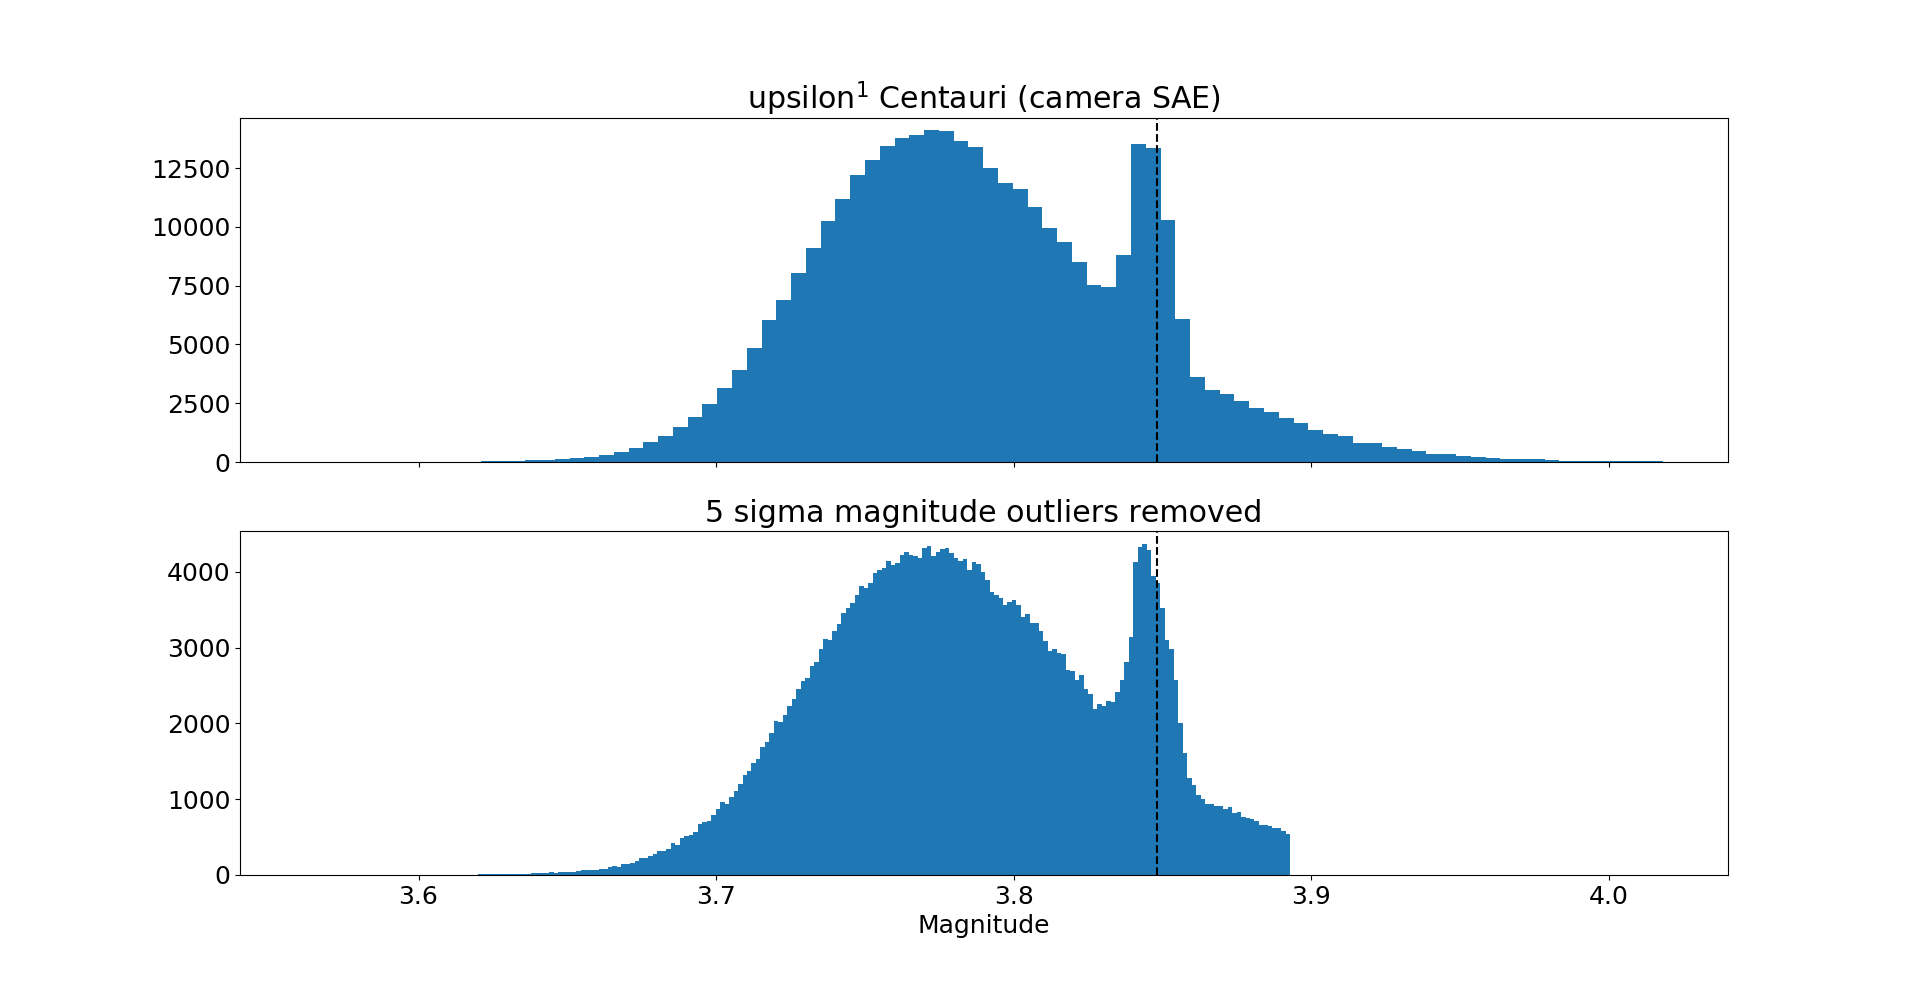
\includegraphics[width=\textwidth]{figures/thesis_histogram.png}
    \caption{Histograms showing the data before and after removing $5\sigma$ magnitude outliers. 200 bins were used for both histograms. The bRing catalogue magnitude value is 3.848 for this star, indicated by the dashed vertical line. The horizontal axis shows the magnitude. The ASCC-number for upsilon$^1$ Centauri is 1959875.}
    \label{hist}
\end{figure}
Another flaw in the data is that the values of the apparent magnitudes may not be accurate compared to other sources. An error remains in the calibration of the magnitudes, and therefore both absolute magnitude values as well as relative changes in magnitude are not completely accurate.
This is because the mean magnitude of the star is fixed to the visual magnitude in the bRing catalogue \citep{Talens_2018}, which is not always correct. The overall shape of fluctuations in magnitude is relatively good, but to determine the depth of transits and periods, follow-up observations are needed.

Furthermore, for the eastern Australian camera, the magnitude of some stars reaches values around $10^{19}$ or higher on one day, which are clearly too extreme. This could be caused by some error in the measurements. The scattering is reduced by removing the 100$\sigma$ magnitude outliers. This high value is chosen, because a smaller value would remove some of the good data points. 

Intrapixel variations were neglected in the data reduction. These sinusoidal modulations are caused by the interline design of the CCDs \citep{Talens_2018}. The intrapixel variations cause noise in the light curves, but are too complex to remove in this research.

The brightest stars which are visible high in the sky have less data points in general. The data at the beginning and end of the night is sufficient to use in the light curves, but the data in the middle of the night cannot be used. These data points are usually saturated, because the star is at its brightest when it is positioned high in the sky.

In contrast, less bright stars which have a declination close to the horizon have fewer data points than stars higher in the sky. This is because they are visible for a smaller amount of time each night. The amount of data points observed still differs for each camera, because of the different locations of the cameras. Overall, the South African eastern camera contains the most data points per star. This is why we mostly use this camera to present the light curves.

\subsection{Detrending}
After detrending the calibrated data, the mean magnitude of the stars is zero. For variable stars this is prevented by adding the offset of the period back into the detrended data. To fix the mean for the stars which are not variable, the mean should be calculated from the data after data reduction is completed, but before detrending is performed. This mean should then be added to the detrended data. However, calculating the mean from the calibrated data does not return the most accurate magnitude value, because of the values from the bRing database mentioned in \ref{sec:discdatared}.

Stars with no known periods were assumed to be non-variable stars and detrended as such. Possible undiscovered periods can be found by using the data available before detrending.
%
Variable stars with a period longer than 500 days were not detrended for their period. If an eclipse is visible in the light curve, it can only show up for a maximum of one time, which means detrending would not have an effect.
%
Pulsating stars with a period below one day were also detrended as non-variable stars. These short periods of a few hours are not visible in the Lomb-Scargle periodograms. The true period could be dominated by systematic effects within one day which cause stronger signals. This is because after detrending, periodic signals of a fraction of a day still remain. Periodic signals of a multiple of one day still remain as well. These signals should be handled carefully when searching for variability in a light curve.
%
No detrending was conducted for the sidereal period of the moon, which is about 27.3 days. This peak is very rarely observed in periodograms. If this peak is still found, it should be treated especially carefully, because we did not remove this signal in the detrending process.

\subsection{Searching for periodic signals}
Periodograms could not be made for all 157 stars, because this process takes a long time. This means that undiscovered periodic signals may still remain in the light curves.

Variable stars with an irregular period are hard to identify by looking at periodograms. Multiple peaks can be found, but period folding does not show a clear shape in the light curve.

Not all signals indicate a true period.
When a period is visible as a signal, a signal will also be visible at multiples of this period. For eclipsing binaries, half of the period may be detected as a signal, due to the overlapping of the primary and secondary period.
%
Lomb-Scargle signals around one year should also be treated carefully when examining periodograms. Usually a broad signal is detected around this period, because large gaps of data overlap. These gaps exist simply because the star is not visible on the sky for several months.

Likewise, a dip in the light curve of a star does not always mean a celestial body moves in front of a star. This drop could be the result of an unclean lens or clouds moving in front of the camera, for example. By looking at data from a different camera or nearby stars using the same camera this theory could be tested. If the dip is not present in the data taken by other cameras, there is no transit occurring. If the light curves of nearby stars show the same drop, the dip is caused by systematic effects. This means there is no actual transit.

For the two stars in the data set most similar to the sun, delta Pavonis and beta Hydri, a search for exoplanets was conducted using TLS. However, no signals were found.


\subsection{Results}
The BRing User Reduction Pipeline (BURP) was created by Remko Stuik to calibrate data of stars observed by the bRing cameras. Using \texttt{burp.detrend}, the data is calibrated and light curves are made. However, BURP does not create proper light curves of stars with $m_V < 4$. A comparison between a light curve created with our calibration and \texttt{burp.detrend} is shown in \ref{burp}. A large amount of scattered data points is still visible in the second plot, particularly below the average magnitude. This means that there are still steps of the data reduction which need to be performed to remove these.
%
In \ref{burpzoom} the light curves are displayed on a daily scale. The values of the vertical axes do not correspond, but the relative scale does. The \texttt{burp.detrend} plot displays a wider range of magnitude compared to the first plot. This range could be visible because the removal of trends during the detrending process is not executed properly for these stars. These figures show that the calibration of light curves is possible if the calibration is conducted differently, as described in \ref{sec:methods}. 

\begin{figure}
    \centering
    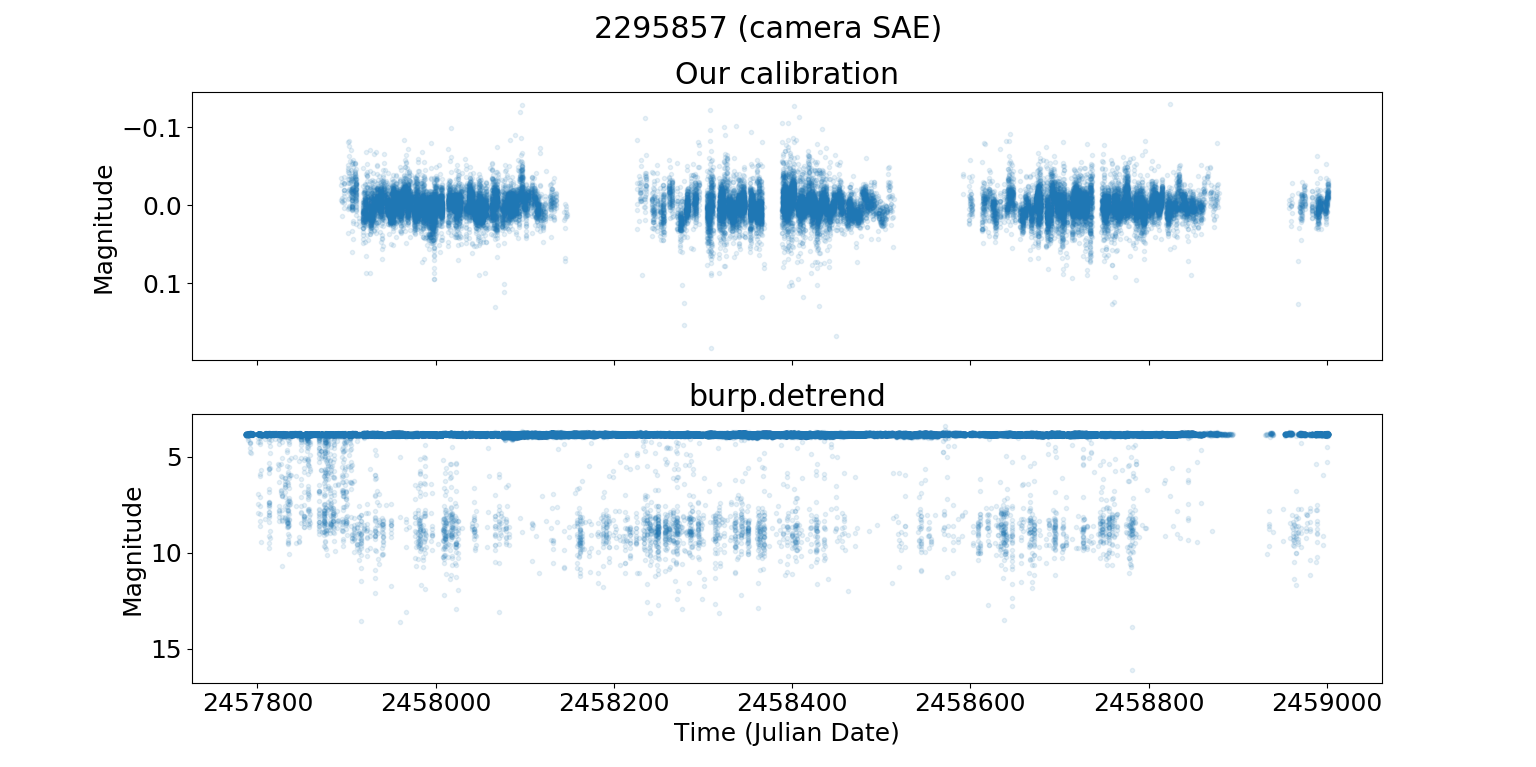
\includegraphics[width=\textwidth]{figures/burpdetrend.png}
    \caption{This figure shows two light curves of a star with ASCC-number 2295857. The first plot shows the light curve created using our calibration and the second plot shows the light curve using the calibration of BURP. The time in Julian Date is displayed on the horizontal axis and the apparent magnitude is displayed on the vertical axis.}
    
    \label{burp}
\end{figure}
\begin{figure}
    \centering
    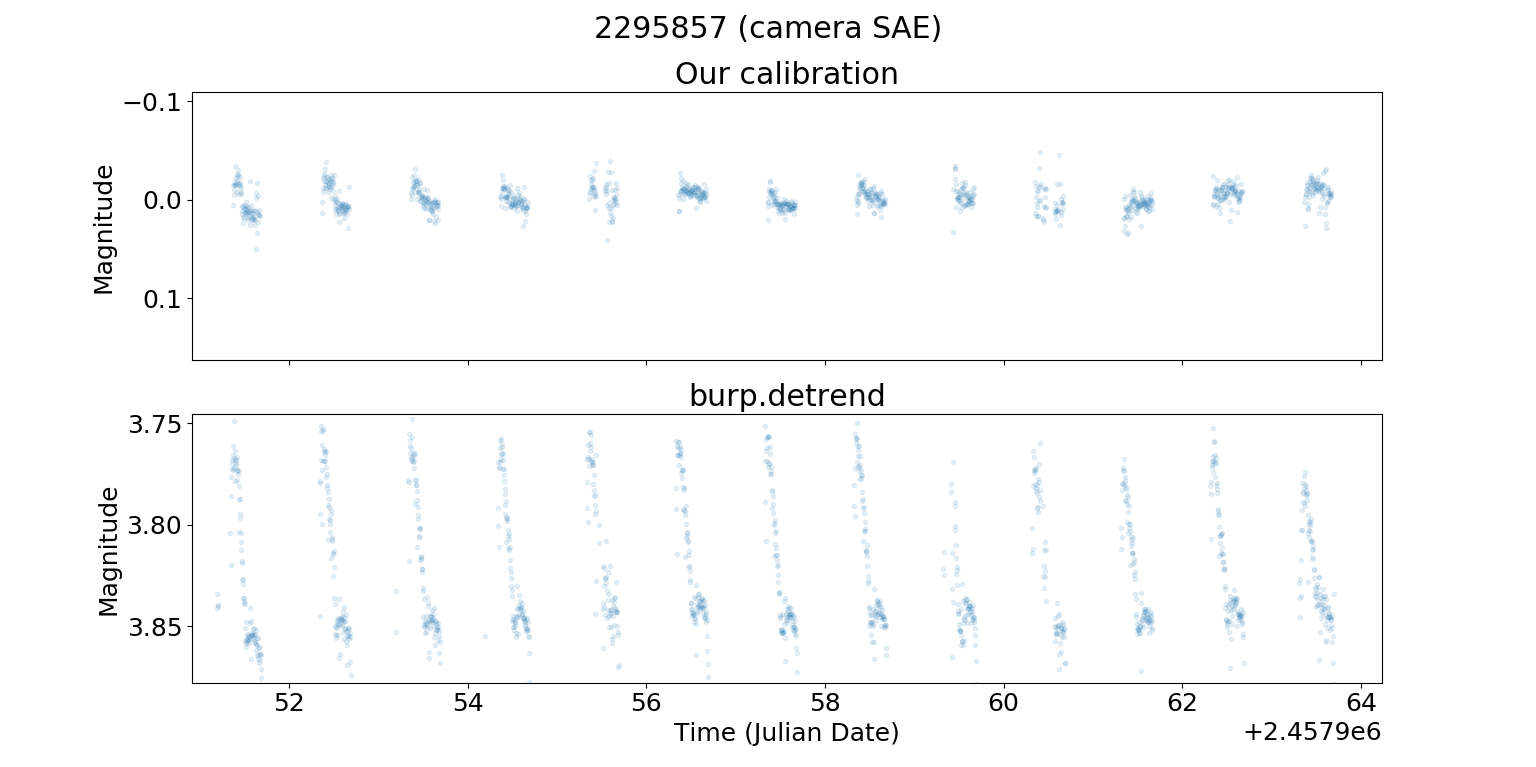
\includegraphics[width=\textwidth]{figures/burpdetrend_zoom.png}
    \caption{This figure shows the difference between our method of calibration and the method of burp. The light curve is shown on a daily scale and both plots have a corresponding vertical scale. The time in Julian Date is displayed on the horizontal axis and the apparent magnitude is displayed on the vertical axis.}
    \label{burpzoom}
\end{figure}

The light curves of the two brightest stars in our data set, Canopus (\ref{Canopus}) and Rigil Kentaurus (\ref{Rigil_Kentaurus}), contain bright peaks of scattered data points. This could be the result of overcorrecting the data affected by clouds, since these peaks occur mostly at very cloudy days.

In the light curve of Hadar (\ref{Hadar}) the brightness seems to fade at the end of a block of data, directly before the star is not visible for a few months. This dip in brightness is probably caused by a lack of calibration. For several stars, it seems the first and last few days of data should be removed because of this inaccuracy.



%We used the data of the eastern South African camera to compute the periods and uncertainties of six variable stars. The uncertainties were computed by dividing the period by the total number of periods present in the data set. The accuracies of the signals could be improved by combining the signals measured by all cameras.\\
%For beta Doradus (\ref{bet_Dor_fold}), a Delta Cephei, we find a period of 9.84 $\pm$ 0.09 days. This is in accordance with a period 9.8426 days according to \cite{Samus_2004}.\\
%For zeta Phoenicis (\ref{zet_Phe_fold}), an eclipsing binary, we find a period of 1.670 $\pm$ 0.002 days with a SDE of 100.3, which is very high. This is similar to 1.6697671 days as stated in \cite{Samus_2004}.\\
%We find a period of 2.943 $\pm$ 0.008 days for alpha Doradus (\ref{alf_Dor_fold}). \cite{Dubath_2011} shows a period of 2.943 days for this rotating star as well.\\
%The second Delta Cephei, l Carinae (\ref{l_Car_fold}), shows a period of 35.6 $\pm$ 1.2 days. This is close to the 35.53584 days as in \cite{Samus_2004}.\\
%Mu$^1$ Scorpii (\ref{mu_Sco_fold}) is a Beta Lyrae-type eclipsing binary, for which we find a period of 1.446 $\pm$ 0.002 days with a SDE of 41.3. This result is in accordance with \cite{Samus_2004}, where a period of 1.44626907 days is stated.\\
%For the eclipsing binary delta Velorum (\ref{del_Vel_fold}), we find a period of 45.2 $\pm$ 2.0 days with a SDE of 3.8. This agrees with the period of 45.15 days as reported by \cite{Pribulla_2011}. The peak does not cross the threshold value of SDE $>$ 6, however. This could be because TLS was meant to be used for transits, and the eclipses have a different shape. This is also our longest period, making it harder to detect. \\
%The period folds of both l Carinae (\ref{l_Car_fold}) and delta Velorum (\ref{del_Vel_fold}) show that longer periods can be detected in the data measured by the bRing instrument. This was not possible for stars brighter than magnitude 4 before bRing was introduced, because not enough data existed of these stars. As a consequence, no long periods could be detected without bRing.

\subsection{Future research}
In the future, the data reduction of the bright stars should be perfected. There are still a few errors in the data which should be fixed. For example, some invalid values remain.

The bRing cameras collect new raw data every day. This means that more calibration will be needed to polish the data collected after this research.

For the first time, long-term light curves have been made for stars brighter than magnitude 4. The light curves produced in this research can be used to determine variability in bright stars' emission by searching for periodic signals. The periodic signals discovered in the bRing data can be studied in more detail using different telescopes.

Furthermore, the shapes of the periods of variable stars brighter than magnitude 4 can now be made visible in a period folded light curve. This could tell us more about the properties of these variable stars.

Moreover, fake transit signals could be inserted in the light curves to determine the boundary conditions of a detectable exoplanet. 



\section{Conclusion}
\label{sec:conclusion}
For the first time, long-term light curves for the 157 brightest stars ($m_V < 4$) in the southern hemisphere ($\delta \leq -30^o$) were created.
The data was collected by the bRing cameras, after which data reduction and detrending was applied. After the calibration, a search for periodic signals in the light curves was conducted. For six variable stars, the periods were found: 
\begin{itemize}
    \item Beta Doradus, a Delta Cephei with a period of $9.84 \pm 0.09$ days.
    \item Zeta Phoenicis, an eclipsing binary with a period of $1.670 \pm 0.002$ days.
    \item Alpha Doradus, a rotating star with a period of $2.943 \pm 0.008$ days.
    \item L Carinae, a Delta Cephei with a period of $35.6 \pm 1.2$ days.
    \item Mu$^1$ Scorpii, a Beta Lyrae-type eclipsing binary with a period of $1.446 \pm 0.002$ days.
    \item Delta Velorum, an eclipsing binary with a period of $45.2 \pm 2.0$ days.
\end{itemize}
The light curves are most suitable for finding variability in the stars' emissions, especially for long periods ($>$ 1 day). The light curves produced in this research could lead to the discovery of exoplanets or stellar companions around the brightest stars in the sky.


\section{Conclusions}

   \begin{enumerate}
      \item asdf
      \item asdf
   \end{enumerate}

\begin{acknowledgements}

This research has used the SIMBAD database, operated at CDS, Strasbourg, France \citep{wenger2000}.
%
This work has used data from the European Space Agency (ESA) mission {\it Gaia} (\url{https://www.cosmos.esa.int/gaia}), processed by the {\it Gaia} Data Processing and Analysis Consortium (DPAC, \url{https://www.cosmos.esa.int/web/gaia/dpac/consortium}).
%
To achieve the scientific results presented in this article we made use of the \emph{Python} programming language\footnote{Python Software Foundation, \url{https://www.python.org/}}, especially the \emph{SciPy} \citep{virtanen2020}, \emph{NumPy} \citep{numpy}, \emph{Matplotlib} \citep{Matplotlib}, \emph{emcee} \citep{foreman-mackey2013}, and \emph{astropy} \citep{astropy_1,astropy_2} packages.
%
This publication makes use of VOSA, developed under the Spanish Virtual Observatory project supported by the Spanish MINECO through grant AyA2017-84089.
%
This publication makes use of VOSA, developed under the Spanish Virtual Observatory\footnote{\url{https://svo.cab.inta-csic.es}} project funded by MCIN/AEI/10.13039/501100011033/ through grant PID2020-112949GB-I00.
%
VOSA has been partially updated by using funding from the European Union's Horizon 2020 Research and Innovation Programme, under Grant Agreement 776403 (EXOPLANETS-A). 
%
\end{acknowledgements}

\bibliographystyle{aa}
\bibliography{bib}

\end{document}
